\chapter{Marco Teórico}\label{ch:Marco Teórico}
En este capítulo se presentará la teoría necesaria para el desarrollo del presente proyecto. Comenzaremos explorando la historia y evolución de las series de Fourier, se detallarán las fórmulas matemáticas para comprender la descomposición de funciones periódicas en sumas de senos y cosenos, resaltando los conceptos de coeficientes de Fourier. Además, se presentan las tecnologías necesarias para la elaboración del proyecto.

\section{Origen e historia de las series de Fourier}
Uno de los problemas del que se ocuparon los matemáticos del siglo XVIII es el que se conoce con el nombre del \textit{problema de la cuerda vibrante}. Este problema fue estudiado por D’Alambert y Euler (usando el método de propagación de las ondas) y un poco más tarde, concretamente en 1753, por Daniel Bernoulli. La solución dada por este difería de la proporcionada por los anteriores y consistió básicamente en expresar la solución del problema como superposición (en general infinita) de ondas sencillas. 
\newline
Las ideas de Bernoulli fueron aplicadas y perfeccionadas por Fourier, en 1807, en el estudio de problemas relacionados con la conducción del calor. Quedaron plasmadas por escrito en el libro clásico \emph{Théorie analytique de la chaleur}, publicado en 1822. Los razonamientos realizados por Fourier en este libro plantearon de manera inmediata numerosas controversias y cuestiones que han tenido una influencia significativa en la historia de la Matemática ~\cite{historia-alambert-fourier-euler}.

\subsection{El problema de la cuerda oscilante}

El problema de la cuerda vibrante, que surge con frecuencia en fenómenos físicos oscilatorios, puede describirse de la siguiente manera: Supongamos una cuerda flexible y tensa, cuyos extremos están fijados en los puntos $(0,0)$ y $(\ell, 0)$ sobre el eje horizontal. Si la cuerda se desplaza de modo que su forma inicial corresponde a la curva definida por $y = f(x)$ y luego se suelta, la pregunta es: ¿cuál será el movimiento resultante de la cuerda?
\newline
Los desplazamientos de la cuerda siempre se encuentran en un mismo plano, y el vector desplazamiento es perpendicular en cualquier momento. Para describir este movimiento se utiliza una función $u(x, t)$, donde $u(x, t)$ representa el desplazamiento vertical de la cuerda en la posición $x$ (con $0 \leq x \leq \ell$) y en el instante $t$ (con $t \geq 0$). El problema es determinar $u(x, t)$ a partir de $f(x)$ ~\cite{weinbergerEDP}.

\subsubsection{D’Alambert y Euler}
El primer matemático que propuso un modelo adecuado para este problema fue Jean Le Rond D’Alambert ~\cite{unal_52162}. Bajo diversas hipótesis (asumiendo, por ejemplo, que las vibraciones son ``pequeñas''), en 1747 D’Alambert dedujo la ecuación de onda en la siguiente forma:

\begin{equation} \label{eq1}
	\begin{split}
		\frac{\partial^2 u(x,t)}{\partial t^2} &=  \frac{\partial^2 u(x,t)}{\partial x^2}, \quad 0 < x < \ell, \ t > 0 \\
	\end{split}
\end{equation}
en donde:
\begin{itemize}
	\item \( u(x,t) \): Es la función que describe el desplazamiento de la onda en función de la posición \( x \) y el tiempo \( t \).
	\item \( \frac{\partial^2 u(x,t)}{\partial t^2} \): Segunda derivada parcial de \( u(x,t) \) respecto al tiempo \( t \), que representa la aceleración del desplazamiento de la onda.
	\item \( \frac{\partial^2 u(x,t)}{\partial x^2} \): Segunda derivada parcial de \( u(x,t) \) respecto a la posición \( x \), que describe la curvatura espacial de la onda.
\end{itemize}

 y esta debe satisfacer las condiciones siguientes:

\begin{equation} \label{eq2}
	\begin{split}
		u(x,0) &= f(x), \quad 0 \leq x \leq \ell \\
		\frac{\partial u(x,0)}{\partial t} &= 0, \quad 0 \leq x \leq \ell \\
		u(0,t) &= u(\ell,t) = 0, \quad t \geq 0.
	\end{split}
\end{equation}


En donde la primera ecuación establece la posición inicial de la cuerda, mientras que la segunda indica que la velocidad inicial de la cuerda es cero (recordando que, una vez desplazada a la posición $f(x)$, la cuerda es liberada). La última condición expresa que, para cualquier tiempo, los extremos de la cuerda permanecen fijos. En la figura \ref{fig:cuerda-vibrante} La variable $u = u(x,t)$ mide el desplazamiento sobre la vertical a tiempo $t > 0$ en la posición $x \in [0,\ell]$.

\begin{figure}[h]
	\centering
	
	\begin{tikzpicture}[scale=1.0]
		% Ejes coordenados
		\draw[->,ultra thick] (-0.5,0) -- (7,0) node[right] {$x$};
		\draw[->,ultra thick] (0,-1) -- (0,2) node[above] {$u(x,t)$};
		
		% Extremos fijos en x=0 y x=L
		\draw[thick] (0,0) circle (0.05) node[below] {$x=0$};
		\draw[thick] (6,0) circle (0.05) node[below] {$x=\ell$};
		
		% Desplazamiento inicial de la cuerda
		\draw[domain=0:6,smooth,variable=\x,guinda,thick] plot ({\x},{1.8*sin(180*\x/6)});
		
		% Etiqueta de la cuerda
		\node[above,guinda] at (3,1.9) {$u(x,0) = f(x)$};
		
		% Condiciones de contorno (Movidas hacia arriba para evitar superposición)
		\draw[<-] (0,0.1) -- (-0.5,0.4) node[left] {$u(0,t)=0$};
		\draw[<-] (6,0.1) -- (6.5,0.4) node[right] {$u(\ell,t)=0$};
		
		% Indicación de tiempo inicial
		\node at (3,-0.8) {$t = 0$};
		
		% Flecha de tiempo (opcional)
		% \draw[->] (6.5,1) -- (6.5,1.5) node[right] {$t$ aumenta};
	\end{tikzpicture}
	\caption[Ilustración del problema de la cuerda vibrante.] {Ilustración del problema de la cuerda vibrante. \textit{Fuente: Elaboración propia} }
	\label{fig:cuerda-vibrante}  % Etiqueta para la figura
\end{figure}
%https://teorica.fis.ucm.es/pparanda/EDPdf/EDPviejas/ppedp6.pdf

Y apartir de esto, construyó la solución ~\cite{demostracion-onda}:

\begin{equation}\label{eq3}
	u(x,t) =   F\left( x+t \right) + G\left( x-t \right)
\end{equation}

Que, estando sujeta a las condiciones de frontera \ref{eq2} se podía reducir a ~\cite{demostracion-onda}:

\begin{equation}\label{eq4}
	u(x,t) =   F\left( x+t \right) + F\left( x-t \right)
\end{equation}

siempre y cuando la función \( F \) fuese periódica, impar y diferenciable en todas partes. D’Alambert demostraba con esto que la ecuación de onda admitía “un número infinito de soluciones”. \newline 

Euler entra en escena al criticar varias de las suposiciones que D'Alambert hiciera para encontrar su solución. Una de particular interés es la de suponer que la forma inicial de la curva o cuerda era continua y diferenciable “como una anguila”. Esta suposición para Euler, le quitaba generalidad a la solución de D' Alambert pues omitía funciones, notablemente la que representa una cuerda al
ser pulsada, como se muestra en la figura \ref{fig:cuerda-vibrante}.
Euler derivó una ecuación de onda ligeramente más general que la de D'Alembert \ref{eq1}:
\begin{equation}\label{eq5}	
	\frac{1}{c^2} \frac{\partial^2 u(x,t)}{\partial t^2} = \frac{\partial^2 u(x,t)}{\partial x^2} 
\end{equation}

con la solución ~\cite{demostracion-onda}:

\begin{equation}\label{eq6}	
	u(x,t) = F(x+ct) + G(x-ct)
\end{equation}

que con las mismas condiciones de frontera resulta en ~\cite{demostracion-onda}:

\begin{equation}\label{eq7}	
	u(x,t) = F(x+ct) + F(x-ct)
\end{equation}


Euler argumentaba, a diferencia de D'Alembert, que la función \( F \) quedaba determinada por la posición y velocidad inicial de la cuerda. Si denotamos por \( w(x) \) y \( v(x) \) a éstas, respectivamente, entonces la solución puede representarse como:


\begin{equation}\label{eq8}	
	u(x,t) = \frac{1}{2} \left( w(x+ct) + w(x-ct) + \frac{1}{c} \int_{x-ct}^{x+ct} v(s) ds \right)
\end{equation}

Las funciones \( w \) y \( v \) podían ser arbitrarias (en el sentido que podían representar cualquier curva que pudiera “dibujarse a mano”) e incluía, implícitamente, a la curva “triangular” de la figura. Como dicen los autores ~\cite{bernoulli_Mechanics} a D'Alembert no le quitaba el sueño sacrificar realismo físico por pureza matemática; Euler, por el contrario, usaba la realidad física para contraargumentar la generalidad de las soluciones obtenidas por el francés aunque su interés no fuera tanto realismo físico sino la generalidad de las soluciones admitidas por la ecuación de onda.

\subsubsection{Bernoulli}
Otra manera de obtener la solución del problema \ref{eq1}, distinta a la de sus distinguidos interlocutores, fue propuesta por Daniel Bernoulli en 1753 ~\cite{bernoulli_Mechanics} La idea clave es obtener la solución de \ref{eq1} como superposición de ondas más sencillas, concretamente aquellas que son de la forma ~\cite{springer1999Physics}:

\begin{equation}\label{eq9}	
	u(x) = \alpha \sin \frac{\pi x}{\ell} + \beta \sin \frac{2\pi x}{\ell} + \gamma \sin \frac{3\pi x}{\ell} + \delta \sin \frac{4\pi x}{\ell} + \dots
\end{equation}

que incorporaban el hecho experimental de que cualquier modo de vibración de una cuerda puede obtenerse superponiendo modos vibratorios simples representados por cada término. Estas funciones representan, para \( n = 1 \), el modo fundamental, y para \( n > 1 \) , sus armónicos. De esta manera, cualquier vibración de la cuerda puede describirse como una superposición de estos armónicos, como se puede ver en la figura \ref{fig:armonicos_cuerda}.

\begin{figure}[h]
	\centering
	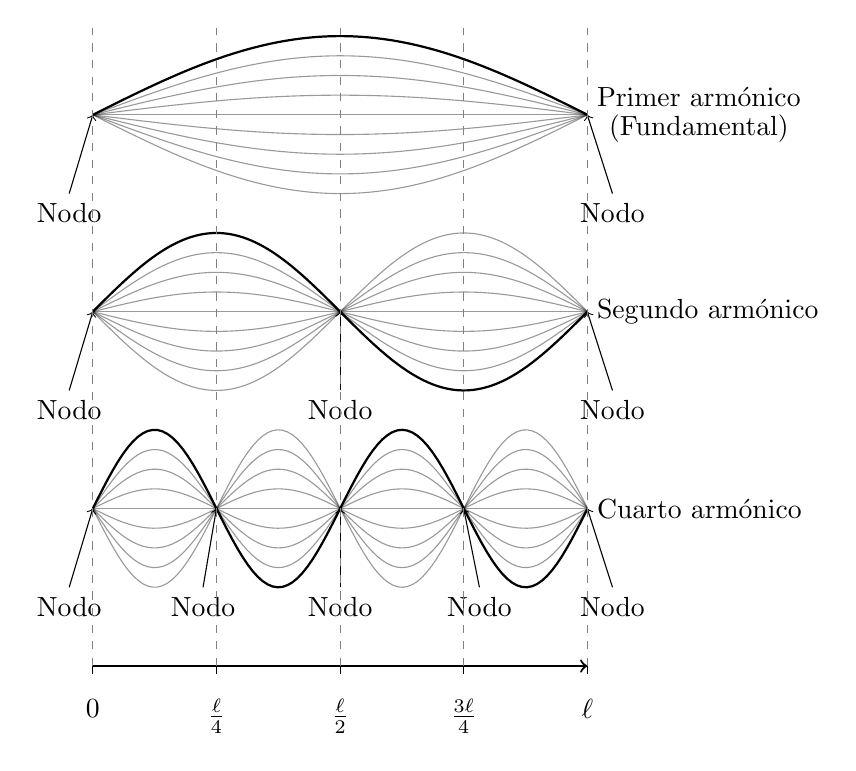
\begin{tikzpicture}[xscale=2]
		
		% Primera onda (n=1)
		\draw[thick] plot[domain=0:3.14, samples=100] (\x,{sin(\x r)});
		\draw [opacity = 0.4] plot[domain=0:3.14, samples=100] (\x,{0.75*sin(\x r)});
		\draw [opacity = 0.4] plot[domain=0:3.14, samples=100] (\x,{0.5*sin(\x r)});
		\draw [opacity = 0.4] plot[domain=0:3.14, samples=100] (\x,{0.25*sin(\x r)});
		\draw [opacity = 0.4] plot[domain=0:3.14, samples=100] (\x,{0*sin(\x r)});
		\draw [opacity = 0.4] plot[domain=0:3.14, samples=100] (\x,{-0.5*sin(\x r)});
		\draw [opacity = 0.4] plot[domain=0:3.14, samples=100] (\x,{-0.25*sin(\x r)});
		\draw [opacity = 0.4] plot[domain=0:3.14, samples=100] (\x,{-0.75*sin(\x r)});
		\draw [opacity = 0.4] plot[domain=0:3.14, samples=100] (\x,{-sin(\x r)});
		\node[right] at (3.14, 0) {\shortstack{Primer armónico \\ (Fundamental)}};
		
		
		\draw[->] (-0.15, -1) node[below] {Nodo} -- (0, 0);
		\draw[->] (3.3, -1) node[below] {Nodo} -- (3.14, 0);
		
		
		% Segunda onda en la parte inferior (misma onda desplazada hacia abajo)
		\begin{scope}[shift={(0,-2.5)}] % Mueve todo el segundo gráfico hacia abajo
			\draw[thick] plot[domain=0:3.14, samples=100] (\x,{sin(2*\x r)});
			\draw [opacity = 0.4] plot[domain=0:3.14, samples=100] (\x,{0.75*sin(2*\x r)});
			\draw [opacity = 0.4] plot[domain=0:3.14, samples=100] (\x,{0.5*sin(2*\x r)});
			\draw [opacity = 0.4] plot[domain=0:3.14, samples=100] (\x,{0.25*sin(2*\x r)});
			\draw [opacity = 0.4] plot[domain=0:3.14, samples=100] (\x,{0*sin(2*\x r)});
			\draw [opacity = 0.4] plot[domain=0:3.14, samples=100] (\x,{-0.5*sin(2*\x r)});
			\draw [opacity = 0.4] plot[domain=0:3.14, samples=100] (\x,{-0.25*sin(2*\x r)});
			\draw [opacity = 0.4] plot[domain=0:3.14, samples=100] (\x,{-0.75*sin(2*\x r)});
			\draw [opacity = 0.4] plot[domain=0:3.14, samples=100] (\x,{-sin(2*\x r)});
			\node[right] at (3.14, 0) {Segundo armónico};
			
			\draw[->] (-0.15, -1) node[below] {Nodo} -- (0, 0);
			\draw[->] (1.57, -1) node[below] {Nodo} -- (1.57, 0);
			\draw[->] (3.3, -1) node[below] {Nodo} -- (3.14, 0);
		\end{scope}
		
		
		% Segunda onda en la parte inferior (misma onda desplazada hacia abajo)
		\begin{scope}[shift={(0,-5)}] % Mueve todo el segundo gráfico hacia abajo
			\draw[thick] plot[domain=0:3.14, samples=100] (\x,{sin(4*\x r)});
			\draw [opacity = 0.4] plot[domain=0:3.14, samples=100] (\x,{0.75*sin(4*\x r)});
			\draw [opacity = 0.4] plot[domain=0:3.14, samples=100] (\x,{0.5*sin(4*\x r)});
			\draw [opacity = 0.4] plot[domain=0:3.14, samples=100] (\x,{0.25*sin(4*\x r)});
			\draw [opacity = 0.4] plot[domain=0:3.14, samples=100] (\x,{0*sin(4*\x r)});
			\draw [opacity = 0.4] plot[domain=0:3.14, samples=100] (\x,{-0.5*sin(4*\x r)});
			\draw [opacity = 0.4] plot[domain=0:3.14, samples=100] (\x,{-0.25*sin(4*\x r)});
			\draw [opacity = 0.4] plot[domain=0:3.14, samples=100] (\x,{-0.75*sin(4*\x r)});
			\draw [opacity = 0.4] plot[domain=0:3.14, samples=100] (\x,{-sin(4*\x r)});
			\node[right] at (3.14, 0) {Cuarto armónico};
			
			% Flechas hacia los nodos
			\draw[->] (-0.15, -1) node[below] {Nodo} -- (0, 0);
			\draw[->] (0.7, -1) node[below] {Nodo} -- (0.785, 0);
			\draw[->] (1.57, -1) node[below] {Nodo} -- (1.57, 0);
			\draw[->] (2.455, -1) node[below] {Nodo} -- (2.355, 0);
			\draw[->] (3.3, -1) node[below] {Nodo} -- (3.14, 0);
		\end{scope}
		
		
		
		\begin{scope}[shift={(0,1)}] 
			% Eje x graduado en múltiplos de pi/4
			\draw[thick, ->] (0,-8) -- (3.14,-8) node[anchor=north] {}; % Eje x
			\foreach \x in {0,0.785,1.57,2.355,3.14} {
				\draw (\x,-8.1) -- (\x,-7.9); % Marcas de tic
			}
			\foreach \x/\label in {0/$0$,0.785/$\frac{\ell}{4}$,1.57/$\frac{\ell}{2}$,2.355/$\frac{3\ell}{4}$,3.14/$\ell$} {
				\draw (\x,-8.3) node[anchor=north] {\label}; % Etiquetas
			}
			
			% Líneas verticales punteadas
			\foreach \x in {0,0.785,1.57,2.355,3.14} {
				\draw[dashed, gray] (\x,-8) -- (\x,0.1); % Líneas punteadas desde el eje x hacia arriba
			}
		\end{scope}
	\end{tikzpicture}
	
	\caption[Ilustración de 3 armónicos y sus nodos de la cuerda al vibrar.] {Ilustración de 3 armónicos y sus nodos de la cuerda al vibrar.\textit{Fuente: Elaboración propia}} 
	\label{fig:armonicos_cuerda}  % Etiqueta para la figura
\end{figure}

Si la solución propuesta por Bernouilli fuese correcta, ello obligaría a que

\begin{equation}\label{eq10}
	u(x, 0) = \sum_{n=1}^{\infty} C_n \sen(nx)
\end{equation}

y por tanto a que

\begin{equation}\label{eq11}
f(x) = \sum_{n=1}^{\infty} C_n \sen(nx), \quad \forall x \in [0, \ell],
\end{equation}

para “una adecuada elección de los coeficientes \( C_n \)”. \newline


Pero esta fórmula no es correcta del todo pues le falta, a cada término, el producto por la función coseno (función del tiempo). Más aún, Bernoulli fue incapaz de mostrar cómo podían obtenerse los coeficientes \( \alpha \), \( \beta \), \( \gamma \), \( \delta \), ... cosa que sí hizo Euler un poco después con el método de integrar la expansión después de multiplicarla por senos o cosenos. Es claro que la solución de Bernoulli no es tan general como la de D’Alembert pero algo que aún el gran Euler no pudo realmente entender es que la solución de Bernoulli permitía funciones iniciales más generales que, a decir de otros autores, fue tema de críticas por parte de Euler a la propuesta de D’Alembert ~\cite{springer1999Physics}.
Bernoulli y Euler mantuvieron una correspondencia epistolar productiva, y se puede afirmar que ambos dependían del otro para realizar su trabajo: Bernoulli necesitaba de Euler para orientar sus estudios matemáticos, mientras que Euler dependía de Bernoulli para comprender los fenómenos físicos que sustentaban su investigación matemática. A pesar de que partían de estudios matemáticos comunes, al final no lograron resolver ni juntos, ni de manera individual, ni desde una perspectiva experimental, donde la matemática jugara un papel metodológico predominante, ni desde el punto de vista matemático donde la física del problema guiara y definiera la teoría. Euler nunca consideró especialmente relevante el trabajo matemático de Daniel Bernoulli, ya que sus métodos eran algo imprecisos, aunque con gran intuición física. Por su parte, Bernoulli tampoco valoraba mucho los estudios matemáticos de Euler, pues estaban distantes de los experimentos. Bernoulli incluso llegó a comentar que Euler ``tomaba sus pruebas de la naturaleza y no de algún principio de análisis '' ~\cite{springer1999Physics}.


\subsection{La ecuación de calor}
Hubo que esperar 54 años hasta que las ideas de Bernoulli fueron tomadas en cuenta por el barón Jean Baptiste-Joseph Fourier, matemático y físico francés, quien, entre otras actividades acompañó a Napoleón, en calidad e científico, en la campaña de éste en Egipto. Allí, como secretario del Instituto de Egipto, hizo gala de gran competencia en diversos asuntos administrativos. ~\cite{almira2017fourier}

\subsubsection{Fourier}
Al regresar a Francia, y como profesor de Análisis de la Escuela Politécnica, Fourier se interesó por la teoría de la conducción del calor en los cuerpos sólidos. En 1807 envió un artículo a la Academia de Ciencias de París, que trataba sobre dicho tema. Más concretamente, Fourier consideró una varilla delgada de longitud dada \( \ell \), cuyos extremos se mantienen a \( 0^\circ \) centígrados y cuya superficie lateral está aislada. Si la distribución inicial de temperatura en la varilla viene dada por una función \( f(x) \) (se supone que la temperatura de la varilla en cada sección transversal de la misma es constante), ¿Cuál será la temperatura de cualquier punto \( x \) de la varilla en el tiempo \( t \)? Suponiendo que la varilla satisface condiciones físicas apropiadas, Fourier demostró que si \( u(x,t) \) representa la temperatura en la sección \( x \) y en el tiempo \( t \), entonces la función \( u \) debe tener la siguiente forma:

\begin{equation} \label{eq12}
	\begin{split}
		\frac{\partial u(x,t)}{\partial t} &= \alpha^2 \frac{\partial^2 u(x,t)}{\partial x^2} , \quad 0 < x < \ell, \ 0 < t < \infty \\
	\end{split}
\end{equation}

en donde: 
\begin{itemize}
	\item \(\frac{\partial u}{\partial t}(x,t)\): Representa la derivada parcial de \(u\) con respecto al tiempo \(t\), es decir, cómo cambia la temperatura \(u(x,t)\) en el punto \(x\) a lo largo del tiempo \(t\).
	\item \(u(x,t)\): Es la función que describe la temperatura en un punto \(x\) en el espacio y en un tiempo \(t\). Depende tanto de la posición espacial \(x\) como del tiempo \(t\).
	
	\item \(\alpha^2\): Es el coeficiente de difusión térmica, que depende del material en cuestión. Este coeficiente es constante y está relacionado con la capacidad del material para difundir el calor. La unidad de \(\alpha\) es metros cuadrados por segundo \((\text{m}^2/\text{s})\).
	\item \(\frac{\partial^2 u}{\partial x^2}(x,t)\): Representa la derivada parcial segunda de \(u\) con respecto a la posición \(x\), es decir, cómo cambia la pendiente (o curvatura) de la temperatura a lo largo del espacio. Esta cantidad indica cómo el calor se distribuye espacialmente.
\end{itemize}

Esta ecuación modela la difusión del calor en un medio a lo largo del tiempo. La derivada en el tiempo \(\left(\frac{\partial u}{\partial t}\right)\) está relacionada con la derivada segunda en el espacio \(\left(\frac{\partial^2 u}{\partial x^2}\right)\), lo que refleja que el cambio en la temperatura con el tiempo depende de cómo está distribuido el calor en el espacio.
y esta debe satisfacer las siguientes condiciones:

\begin{equation} \label{eq13}
	\begin{split}
		u(0,t) &= u(\ell,t) = 0, \quad 0 \leq t \leq \infty \\
		u(x,0) &= f(x), \quad 0 \leq x \leq \ell.
	\end{split}
\end{equation}

\begin{figure}[h]
	\centering
	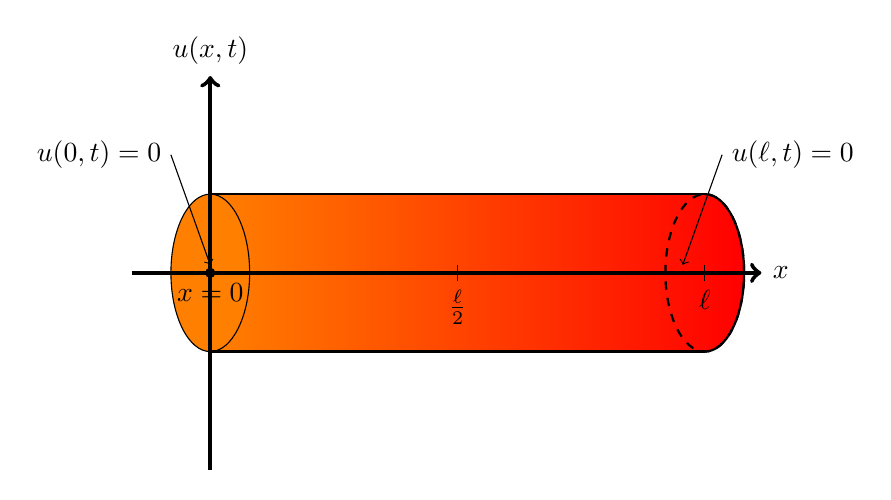
\begin{tikzpicture}
		% Aplicar un sombreado degradado del cilindro (de naranja a rojo)
		\shade[left color=orange, right color=red] (0,1) -- (6.28,1) arc (90:-90:0.5 and 1) -- (0,-1) arc (-90:90:0.5 and 1);
		
		\filldraw [color=orange, draw=black](0,0) ellipse (0.5 and 1);  % Parte delantera del cilindro
		%\shade[left color=orange, right color=red] (0,0) ellipse (0.5 and 1);
		
		% Dibujar las líneas laterales con degradado
		\draw[thick, draw=black] (0,1) -- (6.28,1);
		\draw[thick, draw=black] (0,-1) -- (6.28,-1);
		\draw[thick, draw=black] (6.28,1) arc (90:-90:0.5 and 1);  % Arco frontal
		\draw[dashed, thick, draw=black] (6.28,0) ellipse (0.5 and 1);  % Parte trasera del cilindro
		
		% Dibujar el plano coordenado xy
		\draw[->,ultra thick] (-1,0) -- (7,0) node[right] {$x$};  % Eje x
		\draw[->,ultra thick] (0,-2.5) -- (0,2.5) node[above] {$u(x,t)$};  % Eje y
		
		% Extremos fijos en x=0 y x=L
		\draw[thick] (0,0) circle (0.05) node[below] {$x=0$};
		\draw (3.14,0.1) -- (3.14,-0.1) node[below] {$\frac{\ell}{2}$};
		\draw (6.28,0.1) -- (6.28,-0.1) node[below] {$\ell$};
		
		% Condiciones de contorno (Movidas hacia arriba para evitar superposición)
		\draw[<-] (0,0.1) -- (-0.5,1.5) node[left] {$u(0,t)=0$};
		\draw[<-] (6,0.1) -- (6.5,1.5) node[right] {$u(\ell,t)=0$};
	\end{tikzpicture}
 	\caption[Ilustración del problema de transferencia de calor en una barra de longitud $\ell$.  ]{ Ilustración del problema de transferencia de calor en una barra de longitud $\ell$.  \textit{ Fuente: Elaboración propia} }
	\label{fig:barra-pi}  % Etiqueta para la figura
\end{figure}

La primera condición en \ref{eq12} es una Ecuación en Derivadas Parciales de segundo orden, conocida con el nombre de Ecuación del Calor. La segunda significa que la temperatura, en los extremos de la varilla, se mantiene a \( 0^\circ \) centígrados en cualquier tiempo, mientras que la última relación representa la distribución inicial de temperatura en la varilla considerada.

Partiendo de las ideas de Bernoulli, para la ecuación de ondas, Fourier buscó las soluciones más sencillas que puede presentar la ecuación del calor: aquellas que son de la forma:
\begin{equation} \label{eq14}
	\begin{split}
		u(x,t) = X(x)P(t) \\
	\end{split}
\end{equation}

 Imponiendo la condición de que tales funciones satisfagan, formalmente, dicha ecuación, obtenemos, como en el caso de la ecuación de ondas, los dos problemas siguientes de ecuaciones diferenciales ordinarias ~\cite{demostracion-calor}:
\begin{equation} \label{eq15}
	\begin{split}
		X''(x) + \mu X(x) &= 0, \quad x \in (0, \ell), \ X(0) = X(\ell) = 0 \\
		P'(t) + \mu P(t) &= 0, \quad t > 0
	\end{split}
\end{equation}

Utilizando el método de separación de variables ~\cite{demostracion-calor-feldman}, Fourier propuso que la solución a la ecuación del calor podría expresarse como el producto de dos funciones, una dependiente de la posición \( X(x) \) y otra del tiempo \( P(t) \), como se indica en \eqref{eq13}. Esto descompone la ecuación en dos ecuaciones diferenciales ordinarias: una espacial \eqref{eq15} y una temporal \eqref{eq15}. Fourier resolvió cada una de estas ecuaciones por separado. La solución espacial \( X(t) \) resulta en una serie de funciones sinusoidales que satisfacen las condiciones de frontera en los extremos de la varilla, mientras que la solución temporal \( P(t) \) resulta en exponentes negativos que representan la disipación de calor en el tiempo. Así, disponemos de un procedimiento que nos permite calcular infinitas “soluciones elementales” de la ecuación del calor, a saber, las funciones de la forma \( b_n v_n \), donde \( v_n \) se define como:

\begin{equation} \label{eq16}
	\begin{split}
		v(x,t) = \sin \left( \frac{n \pi}{\ell} x \right) e^{- \alpha^2 \frac{n^2 \pi^2}{\ell^2} k t}
	\end{split}
\end{equation}

Es trivial que, si la distribución inicial de temperatura, \( f \), es algún múltiplo de \( \sen(nx) \) (o una combinación lineal finita de funciones de este tipo), entonces la solución buscada de \eqref{eq16} es un múltiplo adecuado de \( v_n \) (respectivamente, una adecuada combinación lineal de funciones de esta forma).

Ahora bien, \( f(x) \) no es, en general, de la forma justo mencionada, pero, y aquí demostró Fourier, como Bernouilli, una enorme intuición, ¿Será posible obtener la solución \( u(x,t)\) de \eqref{eq16}, para cualquier \( f(x)\) dada, como superposición de las anteriores soluciones sencillas \( v_n \)? Es decir, ¿Será posible elegir adecuadamente los coeficientes \( b_n \) tal que la única solución de \eqref{eq16} sea de la forma:

 
\begin{equation} \label{eq17}
	\begin{split}
		u(x,t) = \sum_{n=1}^{\infty} b_n \sin \left( \frac{n \pi}{\ell} x \right) e^{- \alpha^2 \frac{n^2 \pi^2}{\ell^2} k t}
	\end{split}
\end{equation}

Fourier afirmó en su artículo que esto era correcto. Observemos que nuevamente llegamos a que, entonces, se debe satisfacer la relación \eqref{eq9}. Esto plantea la misma cuestión para dos problemas completamente distintos, el problema \eqref{eq1} y el problema \eqref{eq12}, en donde los coeficientes  \( b_n \) toman la forma:

\begin{equation} \label{eq18}
	\begin{split}
		b_n = \frac{2}{\ell} \int_0^{\ell} f(x) \sin \left( \frac{n \pi x}{\ell} \right) \, dx
	\end{split}
\end{equation}

Los coeficientes \( b_n \) se determinan en función de la distribución inicial de temperatura \( f(x) \) a través de la expresión en \eqref{eq18}, lo que permite que la solución refleje la distribución inicial específica de la varilla. Así, la solución general toma la forma de una serie de Fourier, como se observa en \eqref{eq17}, donde cada término de la serie combina una función sinusoidal en el espacio con un decaimiento exponencial en el tiempo. \newline

El artículo Fourier fue evaluado por Lagrange, Laplace y Legendre y fue rechazado por la Academia Francesa, principalmente debido a la forma en que dedujo la ecuación del calor y por la falta de rigor en sus conclusiones (según la opinión de los académicos mencionados). Sin embargo, los miembros de dicha institución reconocían la relevancia de los problemas relacionados con la propagación del calor, y los resultados teóricos que Fourier presentó mostraban gran concordancia con varios experimentos realizados previamente ~\cite{historia-alambert-fourier-euler}. 

Debido a esto, la Academia estableció un premio sobre el tema. Dicho premio fue otorgado a Fourier en 1812, pero, a pesar de esto, los académicos continuaron criticando la falta de rigor, de modo que, aunque ganó el premio, Fourier no logró publicar su trabajo en la famosa serie “\textit{Mémoires}” de la Academia Francesa. Con gran perseverancia, Fourier continuó trabajando en el tema, y en 1822 publicó su célebre libro \textit{Théorie Analytique de la Chaleur, Firmin Didot, Père et Fils, 1822, París}, donde incluyó gran parte de su artículo de 1812 casi sin modificaciones. Este libro es actualmente una de las obras clásicas en matemáticas ~\cite{historia-alambert-fourier-euler}.

Dos años después, obtuvo el puesto de Secretario de la Academia Francesa, lo que le permitió finalmente publicar su artículo en la serie “\textit{Mémoires}” ~\cite{historia-alambert-fourier-euler}.

\section{Series de Fourier}
Luego de que las soluciones para la ecuación de onda y de calor fueron desarrolladas, Joseph Fourier propuso un nuevo método para expresar funciones periódicas en función de sinusoides. Las bases de lo que hoy conocemos como series de Fourier fueron establecidas por esta propuesta.\newline

A continuación, se describen los conceptos matemáticos en los cuales se basan las series de Fourier, ofreciendo una base firme para entenderlas y aplicarlas en el estudio de funciones que se repiten periódicamente.
\subsection{Funciones Periódicas}
Una función es llamada \textit{función periódica} si existe una constante \( T > 0\) tal que

\begin{equation} \label{eq19}
	\begin{split}
		f(t) = f(t \pm T)
	\end{split}
\end{equation}
para todo valor de \( t \) en el dominio de definición de $f(t)$, donde la constante \( T \) se denomina \textit{periodo} de la función. El periodo también se puede definir como el tiempo transcurrido entre dos puntos equivalentes de una función ~\cite{fourierTolstov}.

Las funciones periódicas aparecen en muchas aplicaciones de matemáticas para problemas de física e ingeniería. Es evidente que la suma, diferencia, producto o cociente de dos funciones con período $T$ también será una función con período $T$ ~\cite{fourierTolstov}.

Si graficamos una función periódica $f(t)$ en un intervalo cerrado $a \leq t \leq a \pm T$, podemos obtener la gráfica completa de $f(t)$ repitiendo periódicamente la porción de la gráfica correspondiente a $a \leq t \leq a \pm T$ \ref{fig:funcion-periodica}.

\begin{figure}[H]
	\centering
	\begin{tikzpicture}[scale=1]
		\begin{axis}[
			axis lines=middle,
			enlargelimits=false,
			width=15cm,
			height=7cm,
			ylabel={\large $f(t)$},
			xlabel={\large $t$},
			xtick={-4*pi, -2*pi, 0, 2*pi, 4*pi},
			xticklabels={$a - 2T$, $a - T$, $a$, $a + T$, $a + 2T$},
			ymin=-4, ymax=4,
			xmin=-4*pi, xmax=4*pi,
			samples=400,
			domain=-4*pi:4*pi,
			axis background/.style={fill=white},
			yticklabels={}, 
			grid=none,
			xticklabel style={yshift=-3cm} % Ajusta el valor según necesites
			]
			
			
			\addplot[guinda, ultra thick] {2 * ((-1)^(1-1)/1 * sin(deg(1*x)) + (-1)^(2-1)/2 * sin(deg(2*x)) + (-1)^(3-1)/3 * sin(deg(3*x)))};    
			
			\addplot[dashed, black, thick] coordinates {(2*pi, -4) (2*pi, 4)};
			\addplot[dashed, black, thick] coordinates {(-2*pi, -4) (-2*pi, 4)};
			\addplot[dashed, black, thick] coordinates {(4*pi, -4) (4*pi, 4)};
			\addplot[dashed, black, thick] coordinates {(-4*pi, -4) (-4*pi, 4)};
			
		\end{axis}
	\end{tikzpicture}
	
		\caption[Gráfica de una función periódica $f(t)$ con periodo $T$.]  {Gráfica de una función periódica $f(t)$ con periodo $T$.\textit{ Fuente: Elaboración propia} }
	\label{fig:funcion-periodica}  % Etiqueta para la figura
\end{figure}
Si $T$ es un período de la función $f(t)$, entonces los números $2T$, $3T$, $4T$, $\dots$ también son períodos. Esto se deduce fácilmente al inspeccionar la gráfica de una función periódica o a partir de la serie de igualdades ~\cite{fourierHsu}
\begin{equation} \label{eq20}
	\begin{split}
		f(t) = f(t \pm T) = f(t \pm 2T) = f(t \pm 3T) = \dots f(t \pm nT), \quad n = 0, \pm1, \pm2, \dots
	\end{split}
\end{equation}
que se obtiene mediante el uso repetido de la condición \eqref{eq19}. Así, si \( T \) es un periodo, también lo es \( nT \), donde \( n \) es cualquier entero positivo, es decir, si existe un periodo, no es único ~\cite{fourierHsu}. Ademas, podemos definir como el \textit{periodo fundamental} \( T_0 \) de \( f(t) \) a el valor positivo más pequeño de \( T \) para el cual se satisface \eqref{eq19}. ~\cite{fourierCinvestav} \newline

Ahora, consideremos la siguiente propiedad de cualquier función \( f(t) \) con período \( T \):

Si \( f(t) \) es integrable en cualquier intervalo de longitud \( T \), entonces es integrable en cualquier otro intervalo de la misma longitud, y el valor de la integral es el mismo. Es decir,

\begin{equation} \label{eq21}
	\int_a^{a+T} f(t) \, dx = \int_b^{b+T} f(t) \, dt
\end{equation}

para cualquier \( a \) y \( b \).

Esta propiedad es una consecuencia directa de la interpretación del área bajo la curva como la integral. De hecho, cada integral de la ecuación anterior representa el área entre la curva \( f(t) \), el eje \( t \), y las líneas verticales en los puntos extremos del intervalo. Las áreas sobre el eje \( t \) se consideran positivas y las áreas bajo el eje \(t\) como negativas. En este caso, las áreas representadas por ambas integrales son iguales debido a la periodicidad de \( f(t) \) ~\cite{fourierTolstov} \ref{fig:area-periodica}.

\begin{figure}
	
	\begin{tikzpicture}[scale=1]
		\begin{axis}[
			axis lines=middle,
			enlargelimits=false,
			width=15cm,
			height=7cm,
			ylabel={\large $f(t)$},
			xlabel={\large $t$},
			xtick={-5*pi/2, -pi/2, pi/4, 9*pi/4},
			xticklabels={\large $a$, $a + T$, $b$, $b + T$},
			ymin=-4, ymax=4,
			xmin=-3*pi, xmax=3*pi,
			samples=400,
			domain=-3*pi:3*pi,
			axis background/.style={fill=white},
			yticklabels={}, 
			grid=none,
			xticklabel style={yshift=-3.2cm, xshift=0} % Ajusta el valor según necesites
			]
			
			% Colorear el área bajo la curva entre a y a+T con patrón
			\addplot [
			draw=none,
			pattern=north east lines, % <-- Cambia fill por pattern
			pattern color=blue,       % <-- Define el color del patrón
			domain=-5*pi/2:-pi/2,
			samples=400,
			] {2 * ((-1)^(1-1)/1 * sin(deg(1*x)) + (-1)^(2-1)/2 * sin(deg(2*x)) + (-1)^(3-1)/3 * sin(deg(3*x)))} \closedcycle;
			
			% Colorear el área bajo la curva entre b y b+T con patrón
			\addplot [
			draw=none,
			pattern=north west lines, % <-- Cambia fill por pattern
			pattern color=red,        % <-- Define el color del patrón
			domain=pi/4:9*pi/4,
			samples=400,
			] {2 * ((-1)^(1-1)/1 * sin(deg(1*x)) + (-1)^(2-1)/2 * sin(deg(2*x)) + (-1)^(3-1)/3 * sin(deg(3*x)))} \closedcycle;
			
			\addplot[guinda, ultra thick] {2 * ((-1)^(1-1)/1 * sin(deg(1*x)) + (-1)^(2-1)/2 * sin(deg(2*x)) + (-1)^(3-1)/3 * sin(deg(3*x)))};    
			
			\addplot[dashed, black, thick] coordinates {(-5*pi/2, -4) (-5*pi/2, 4)};
			\addplot[dashed, black, thick] coordinates {(-pi/2, -4) (-pi/2, 4)};
			\addplot[dashed, black, thick] coordinates {(pi/4, -4) (pi/4, 4)};
			\addplot[dashed, black, thick] coordinates {(9*pi/4, -4) (9*pi/4, 4)};
			
		\end{axis}
	\end{tikzpicture}
	\caption[Gráfica del área bajo la curva de $f(t)$ entre los intervalos desde $a$ hasta $a + T$ y desde $b$ hasta $b + T$. ]{Gráfica del área bajo la curva de $f(t)$ entre los intervalos desde $a$ hasta $a + T$ y desde $b$ hasta $b + T$. \textit{ Fuente: Elaboración propia} }
	\label{fig:area-periodica}  % Etiqueta para la figura
\end{figure}

A partir de ahora, cuando afirmemos que una función \( f(t) \) de período \( T \) es integrable, queremos decir que es integrable en un intervalo de longitud \( T \). Esto implica, a partir de la propiedad recién demostrada, que \( f(t) \) es integrable en cualquier intervalo de longitud finita ~\cite{fourierTolstov}. \newline

Las funciones periódicas más representativas son las funciones trigonométricas \(\sin(t)\) y \(\cos(t)\), ambas con periodo \( T = 2\pi \) (Figura \ref{fig:sen-cos}). Por lo tanto, de acuerdo con \eqref{eq19}, se tiene que \(\sin(t + 2\pi) = \sin(t)\) y \(\cos(t + 2\pi) = \cos(t)\) ~\cite{fourierCinvestav}.

\begin{figure}[H]
	
	\begin{minipage}{0.5\textwidth} % Reducimos el ancho al 48%
		\begin{tikzpicture}[scale=0.46]
			\begin{axis}[
				axis lines=middle,
				grid=both,
				enlargelimits=false,
				width=15cm, % Ancho de la gráfica
				height=13cm, % Altura de la gráfica
				xlabel={\Huge $t$},
				ylabel={\Huge $f(t) = A \sin(t)$},
				xtick={0, 1.5708, 3.1416, 4.7124, 6.2832, 7.8540, 9.4248, 10.9956, 12.5664},
				xticklabels={$0$, $\frac{\pi}{2}$, $\pi$, $\frac{3\pi}{2}$, $2\pi$, $\frac{5\pi}{2}$, $3\pi$, $\frac{7\pi}{2}$, $4\pi$},
				xticklabel style={font=\LARGE},
				ytick={-1.5, -1, -0.5, 0, 0.5, 1, 1.5}, % Gradación de 0.5 en 0.5 en el eje y
				yticklabel style={font=\LARGE},
				ymin=-1.5, ymax=1.5,
				xmin=0, xmax=4*pi,
				samples=400,
				domain=0:4*pi,
				axis background/.style={fill=white}
				]
				
				\addplot[guinda, ultra thick] {( sin(180*x/pi) )};
				
				\addplot[dashed, black, thick] coordinates {(2*pi, -1.5) (2*pi, 1.5)};
				\draw[<->, ultra thick, red] (0,-1.25) -- (2*pi,-1.25) node[midway, below, black] {\LARGE $T$};
				\draw[<->, ultra thick, red] (3*pi/2,0) -- (3*pi/2,-1) node[midway, below right, black, xshift=0.1cm] {\LARGE $A$};
			\end{axis}
		\end{tikzpicture}
	\end{minipage}
	\hspace{0.1cm} % Espacio de 0.5 cm entre las gráficas
	\begin{minipage}{0.5\textwidth} % Reducimos el ancho al 48%
		\begin{tikzpicture}[scale=0.46]
			\begin{axis}[
				axis lines=middle,
				grid=both,
				enlargelimits=false,
				width=15cm, % Ancho de la gráfica
				height=13cm, % Altura de la gráfica
				xlabel={\Huge $t$},
				ylabel={\Huge $f(t) = A \cos(t)$},
				xtick={0, 1.5708, 3.1416, 4.7124, 6.2832, 7.8540, 9.4248, 10.9956, 12.5664},
				xticklabels={$0$, $\frac{\pi}{2}$, $\pi$, $\frac{3\pi}{2}$, $2\pi$, $\frac{5\pi}{2}$, $3\pi$, $\frac{7\pi}{2}$, $4\pi$},
				xticklabel style={font=\LARGE},
				ytick={-1.5, -1, -0.5, 0, 0.5, 1, 1.5}, % Gradación de 0.5 en 0.5 en el eje y
				yticklabel style={font=\LARGE},
				ymin=-1.5, ymax=1.5,
				xmin=0, xmax=4*pi,
				samples=400,
				domain=0:4*pi,
				axis background/.style={fill=white}
				]
				
				\addplot[guinda, ultra thick] {( cos(180*x/pi) )};
				
				\addplot[dashed, black, thick] coordinates {(2*pi, -1.5) (2*pi, 1.5)};
				\draw[<->, ultra thick, red] (0,-1.25) -- (2*pi,-1.25) node[midway, below, black] {\LARGE $T$};
				\draw[<->, ultra thick, red] (pi,0) -- (pi,-1) node[midway, below right, black, xshift=0.1cm] {\LARGE $A$};
			\end{axis}
		\end{tikzpicture}
	\end{minipage}
	\caption[Gráfica de las funciones trigonométricas $sin(t)$ y $cos(t)$.  ]{Gráfica de las funciones trigonométricas $sin(t)$ y $cos(t)$. \textit{ Fuente: Elaboración propia} }
	\label{fig:sen-cos}  % Etiqueta para la figura
\end{figure}

\subsection{Frecuencia}
La relación entre la \textit{frecuencia} \( f \) y el \textit{periodo} \( T \) de una función oscilatoria está dada por
\begin{equation} \label{eq22}
	f = \frac{1}{T}
\end{equation}
lo cual indica el número de oscilaciones de la función por unidad de tiempo. La unidad de medida de la frecuencia es el hertz (Hz). Un hertz quiere decir que una función oscila una vez por segundo ~\cite{fourierCinvestav}. La Figura \ref{fig:seno-diferentes-frecuencias} muestra una función senoidal con tres frecuencias diferentes.

\begin{figure}[H]
	\centering
	\begin{tikzpicture}[scale=0.8]
		\begin{axis}[
			axis lines=middle,
			grid=both,
			enlargelimits=false,
			width=15cm, % Ancho de la gráfica
			height=13cm, % Altura de la gráfica
			xlabel={\large $t$},
			ylabel={\large $f(t)$},
			xtick={0, 0.7854, 1.5708, 2.3562, 3.1416, 3.9269, 4.7124, 5.498, 6.2832},
			xticklabels={\large $0$, $\frac{\pi}{4}$, $\frac{\pi}{2}$, $\frac{3\pi}{4}$, $\pi$, $\frac{5\pi}{4}$, $\frac{3\pi}{2}$, $\frac{7\pi}{4}$, $2\pi$},
			xticklabel style={font=\Large},
			ytick={-1, -0.5, 0, 0.5, 1}, % Gradación de 0.5 en 0.5 en el eje y
			ymin=-2, ymax=1.1,
			xmin=0, xmax=2*pi,
			samples=400,
			domain=0:4*pi,
			axis background/.style={fill=white}
			legend style={at={(0.02,0.98)}, anchor=north west},% Posición ajustada a la esquina superior izquierda
			axis background/.style={fill=white}
			]
			
			\addplot[guinda, ultra thick] {( sin(180*x/pi) )};
			\addlegendentry{1 Hz};
			\addplot[red, ultra thick, dashed] {( sin(360*x/pi) )};
			\addlegendentry{2 Hz};
			\addplot[orange, ultra thick, dotted] {( sin(540*x/pi) )};
			\addlegendentry{3 Hz};
			
			\addplot[dashed, black,  thick] coordinates {(pi, 0) (pi, -4)};
			\addplot[dashed, black,  thick] coordinates {(2*pi/3, 0) (2*pi/3, -4)};
			\addplot[dashed, black,  thick] coordinates {(2*pi, 0) (2*pi, -4)};
			
			\draw[<->, ultra thick, orange] (0,-1.25) -- (2*pi/3,-1.25) node[midway, below, black] {\large $T_1$};
			\draw[<->, ultra thick, red] (0,-1.5) -- (pi,-1.5) node[midway, below, black] {\large $T_2$};
			\draw[<->, ultra thick, guinda] (0,-1.75) -- (2*pi,-1.75) node[midway, below, black] {\large $T_3$};
			
			
		\end{axis}
	\end{tikzpicture}
	\caption[Función $sin(t)$ con diferentes frecuencias]{Función $sin(t)$ con diferentes frecuencias. \textit{Fuente: Elaboración propia}}
	\label{fig:seno-diferentes-frecuencias}  % Etiqueta para la figura
\end{figure}

La \textit{frecuencia angular}, usualmente denotada por \( \omega_0 \), se define como la razón de cambio del desplazamiento angular \( \theta \) durante la oscilación (o rotación) ~\cite{fourierCinvestav}:

\begin{equation} \label{eq23}
	\frac{d\theta}{dt} = \omega_0 = 2 \pi f = \frac{2 \pi}{T}.
\end{equation}

La frecuencia angular se mide comúnmente en radianes por segundo (\( \text{rad/s} \)). La Figura\ref{fig:frecuencia-func-circ} ejemplifica la relación de una onda senoidal en el intervalo \([0, 2\pi]\) con una frecuencia angular \( \omega_0 \). ~\cite{fourierCinvestav}
\begin{figure}[H]
	\begin{minipage}{0.5\textwidth} % Reducimos el ancho al 48%
	\begin{tikzpicture}[scale=0.5]
		\begin{axis}[
			axis lines=middle,
			grid=both,
			enlargelimits=false,
			width=15cm, % Ancho de la gráfica
			height=13cm, % Altura de la gráfica
			xlabel={\huge $t$},
			ylabel={\huge $f(t)$},
			xtick={0, 0.7854, 1.5708, 2.3562, 3.1416, 3.9269, 4.7124, 5.498, 6.2832},
			xticklabels={ $0$, $\frac{\pi}{4}$, $\frac{\pi}{2}$, $\frac{3\pi}{4}$, $\pi$, $\frac{5\pi}{4}$, $\frac{3\pi}{2}$, $\frac{7\pi}{4}$, $2\pi$},
			xticklabel style={font=\huge},
			ytick={-1, -0.5, 0, 0.5, 1}, % Gradación de 0.5 en 0.5 en el eje y
			ymin=-1.1, ymax=1.1,
			xmin=0, xmax=2*pi,
			samples=400,
			domain=0:4*pi,
			axis background/.style={fill=white}
			]
			
			\addplot[guinda, ultra thick] {( sin(180*x/pi) )};
			
			\draw[<->, ultra thick, red] (pi/2,0) -- (pi/2,1) node[midway, below right, black, xshift=0.1cm] {\huge $A$};
		\end{axis}
	\end{tikzpicture}
	\end{minipage}
	\hspace{1cm} % Espacio de 0.5 cm entre las gráficas
	\begin{minipage}{0.5\textwidth} % Reducimos el ancho al 48%
		\scalebox{0.5}{
		\begin{tikzpicture}
			% Draw the circle
			\draw[ultra thick, guinda] (0,0) circle (4cm);
			
			% Draw the axes
			\draw[->] (-4.5,0) -- (4.5,0) node[right] {\huge $0$};
			\draw[->] (0,-4.5) -- (0,4.5) node[above] {\huge $\frac{\pi}{2}$};
			
			% Label the angles
			\node at (-4.5, 0) [left] {\huge $\pi$};
			\node at (0, -4.5) [below] {\huge $\frac{3\pi}{2}$};
			
			% Draw the radius line
			\draw[<->, ultra thick, red] (0,0) -- (2.82,2.82);
			
			% Draw angle
			\draw [thick](1.5,0) arc (0:45:1.5); % Cambia el radio del arco a 0.8 para hacerlo más grande
			\node at (1.8,0.7) {\huge $\theta$};
		\end{tikzpicture}
	}
	\end{minipage}
	\caption[Relación de la frecuencia angular entre la función $sin(t)$ con el circulo unitario.] {Relación de la frecuencia angular entre la función $sin(t)$ con el circulo unitario.\textit{ Fuente: Elaboración propia}  }
	\label{fig:frecuencia-func-circ}  % Etiqueta para la figura
\end{figure}

\subsection{Armónicos}
Las funciones periódicas más representativas son:
\begin{equation}
	f(t) = A \sin(\omega_0 t + \varphi) \quad \text{o} \quad f(t) = A \cos(\omega_0 t + \varphi)
\end{equation}

Cabe señalar que, dado que las funciones seno y coseno solo se diferencian por un deslizamiento de fase, este movimiento podría modelarse usando la función coseno o la función seno, en donde \(A\), \(\omega_0\), y \(\varphi\) son constantes. En una función armónica, la \textit{amplitud} \(A\) representa el valor máximo de la oscilación. La \textit{frecuencia angular} \(\omega_0\) determina la rapidez con la que se realiza la oscilación y viene dada por $\frac{2\pi}{T}$, recordando que $T$ es el periodo de la función, y la \textit{fase inicial} \(\varphi\) indica el desplazamiento de la función en el tiempo al inicio de la observación, es decir, indica con que desfase comienza. \ref{fig:fase-coseno} ~\cite{armonicosOpenStax}. 

\begin{figure}[H]
	\begin{minipage}{0.5\textwidth} % Reducimos el ancho al 48%
		\begin{tikzpicture}[scale=0.5]
			\begin{axis}[
				axis lines=middle,
				grid=both,
				enlargelimits=false,
				width=15cm, % Ancho de la gráfica
				height=13cm, % Altura de la gráfica
				xlabel={\huge $\theta$},
				ylabel={\huge $f(\theta)$},
				xtick={-3.1416, -2.3562, -1.5708, -0.7854, 0, 0.7854, 1.5708, 2.3562, 3.1416, 3.9269, 4.7124, 5.498, 6.2832},
				xticklabels={ $-\pi$, $-\frac{3\pi}{4}$, $-\frac{\pi}{2}$, $-\frac{\pi}{4}$, $0$, $\frac{\pi}{4}$, $\frac{\pi}{2}$, $\frac{3\pi}{4}$, $\pi$, $\frac{5\pi}{4}$, $\frac{3\pi}{2}$, $\frac{7\pi}{4}$, $2\pi$},
				xticklabel style={font=\LARGE},
				ytick={-2, -1, 0, 1, 2}, % Gradación de 0.5 en 0.5 en el eje y
				ymin=-2, ymax=2,
				xmin=-pi, xmax=2*pi,
				samples=400,
				domain=-pi:2*pi,
				axis background/.style={fill=white}
				]
				% Mueve la etiqueta f(t) al lado izquierdo del eje y y la pone en color rojo
				\node at (axis cs:0.4,1.2) {\huge \textcolor{guinda}{$f(\theta) = \cos(\theta)$}};
				\addplot[guinda, ultra thick] {( cos(180*x/pi) )};
			\end{axis}
		\end{tikzpicture}
	\end{minipage}
	\hspace{0.25cm} % Espacio de 0.5 cm entre las gráficas
	\begin{minipage}{0.5\textwidth} % Reducimos el ancho al 48%
		\begin{tikzpicture}[scale=0.5]
			\begin{axis}[
				axis lines=middle,
				grid=both,
				enlargelimits=false,
				width=15cm, % Ancho de la gráfica
				height=13cm, % Altura de la gráfica
				xlabel={\huge $\theta$},
				ylabel={\huge $f(\theta)$},
				xtick={-3.1416, -2.3562, -1.5708, -0.7854, 0, 0.7854, 1.5708, 2.3562, 3.1416, 3.9269, 4.7124, 5.498, 6.2832},
				xticklabels={ $-\pi$, $-\frac{3\pi}{4}$, $-\frac{\pi}{2}$, $-\frac{\pi}{4}$, $0$, $\frac{\pi}{4}$, $\frac{\pi}{2}$, $\frac{3\pi}{4}$, $\pi$, $\frac{5\pi}{4}$, $\frac{3\pi}{2}$, $\frac{7\pi}{4}$, $2\pi$},
				xticklabel style={font=\LARGE},
				ytick={-2, -1, 0, 1, 2}, % Gradación de 0.5 en 0.5 en el eje y
				ymin=-2, ymax=2,
				xmin=-pi, xmax=2*pi,
				samples=400,
				domain=-pi:2*pi,
				axis background/.style={fill=white}
				]
				% Mueve la etiqueta f(t) al lado izquierdo del eje y y la pone en color rojo
				\node at (axis cs:0.4,1.2) {\huge \textcolor{guinda}{$f(\theta) = \cos(\theta + \textcolor{orange}{\varphi})$}};
				\addplot[guinda, ultra thick] {( cos(180*x/pi - 57.2958*pi/2) )};
				\addplot[dashed, black, thick] coordinates {(pi/2, -2) (pi/2, 2)};
				\draw[<->, ultra thick, red, dashed] (axis cs:0,-1) -- (axis cs:pi/2,-1) node[midway, below, black] {\huge $\textcolor{orange}{\varphi}$};
			\end{axis}
		\end{tikzpicture}
	\end{minipage}
	\caption[Una función coseno y la misma función coseno desplazada hacia la izquierda por un ángulo $\varphi$.] {Una función coseno y la misma función coseno desplazada hacia la izquierda por un ángulo $\varphi$.\textit{ Fuente: Elaboración propia}  }
	\label{fig:fase-coseno}  % Etiqueta para la figura
\end{figure}

\subsection{Funciones Pares e Impares}
Más adelante se verá como es que el hecho de que una función $f(t)$  sea par o impar puede ahorrar diversos cálculos, comenzamos definiendo que una función es par si se cumple que: ~\cite{matesAvanzadasZill}

\begin{equation} \label{eq24}
	f(t) = f(-t) , \quad -L < t < L
\end{equation}

En la Figura \ref{fig:funcion-par} se muestra un ejemplo de una función para en donde se puede observar la definición \eqref{eq24}
\begin{figure}[H]
	\centering
	\begin{tikzpicture}[scale=0.5]
		\begin{axis}[
			axis lines=middle,
			grid=both,
			enlargelimits=false,
			width=15cm, % Ancho de la gráfica
			height=13cm, % Altura de la gráfica
			xlabel={\huge $t$},
			ylabel={\huge $f(t)$},
			xtick={-3,-2,-1,0,1,2,3},
			ytick={-3,-2,-1,0,1,2,3},
			xticklabels=\empty, % Elimina los números en el eje x
			yticklabels=\empty, % Elimina los números en el eje y
			ymin=-3, ymax=3,
			xmin=-3, xmax=3,
			samples=400,
			domain=-3:3,
			axis background/.style={fill=white}
			]
			% Agrega etiquetas "t" en x=2 y x=-2
			\node at (axis cs:2,-0.5) {\huge $t$};
			\node at (axis cs:-2,-0.5) {\huge $-t$};
			
			% Dibuja las líneas rojas
			\draw[<->, ultra thick, red, dashed] (axis cs:0,2) -- (axis cs:-2,2);
			\draw[<->, ultra thick, red, dashed] (axis cs:-2,0) -- (axis cs:-2,2);
			\draw[<->, ultra thick, red, dashed] (axis cs:0,2) -- (axis cs:2,2);
			\draw[<->, ultra thick, red, dashed] (axis cs:2,0) -- (axis cs:2,2);
			
			% Agrega la curva azul
			\addplot[guinda, ultra thick] {(x^2 - 2)};
		\end{axis}
	\end{tikzpicture}
	\caption[Función $f(t) = t^{2}$, una función par.]{Función $f(t) = t^{2}$, una función par. \textit{Fuente: Elaboración propia}}
	\label{fig:funcion-par}  % Etiqueta para la figura
\end{figure}

Ahora, decimos que una función es impar si se cumple que: ~\cite{matesAvanzadasZill}
\begin{equation} \label{eq25}
	f(t) = - f(t) , \quad -L < t < L
\end{equation}

En la Figura \ref{fig:funcion-impar} se muestra un ejemplo de una función para en donde se puede observar la definición \eqref{eq25}
\begin{figure}[H]
	\centering
	\begin{tikzpicture}[scale=0.5]
		\begin{axis}[
			axis lines=middle,
			grid=both,
			enlargelimits=false,
			width=15cm, % Ancho de la gráfica
			height=13cm, % Altura de la gráfica
			xlabel={\huge $t$},
			xtick={-3,-2,-1,0,1,2,3},
			ytick={-3,-2,-1,0,1,2,3},
			xticklabels=\empty, % Elimina los números en el eje x
			yticklabels=\empty, % Elimina los números en el eje y
			ymin=-3, ymax=3,
			xmin=-3, xmax=3,
			samples=400,
			domain=-3:3,
			axis background/.style={fill=white}
			]
			% Agrega etiquetas "t" en x=2 y x=-2
			\node at (axis cs:-1.4,0.5) {\huge $t$};
			\node at (axis cs:1.4,-0.5) {\huge $-t$};
			
			% Mueve la etiqueta f(t) al lado izquierdo del eje y
			\node at (axis cs:-0.5,2.744) {\huge $f(t)$};
			\node at (axis cs:0.5,-2.744) {\huge $f(t)$};
			
			% Dibuja las líneas rojas
			\draw[<->, ultra thick, red, dashed] (axis cs:-1.4,-2.744) -- (axis cs:0,-2.744);
			\draw[<->, ultra thick, red, dashed] (axis cs:-1.4,0) -- (axis cs:-1.4,-2.744);
			
			\draw[<->, ultra thick, red, dashed] (axis cs:1.4,2.744) -- (axis cs:0,2.744);
			\draw[<->, ultra thick, red, dashed] (axis cs:1.4,0) -- (axis cs:1.4,2.744);
			
			% Agrega la curva azul
			\addplot[guinda, ultra thick] {(x^3)};
		\end{axis}
	\end{tikzpicture}
	\caption[Función $f(t) = t^{3}$, una función impar]{Función $f(t) = t^{3}$, una función impar. \textit{Fuente: Elaboración propia}}
	\label{fig:funcion-impar}  % Etiqueta para la figura
\end{figure}
Podemos decir entonces que en un intervalo simétrico $-L < t < L$, la gráfica de una función par tiene simetría respecto al eje y, mientras que la gráfica de una función impar tiene simetría en relación con el origen. Además, las funciones pares e impares culpen con los siguientes teoremas ~\cite{matesAvanzadasZill}:
\begin{itemize}
	\item[a)] El producto de dos funciones pares es par.
	\item[b)] El producto de dos funciones impares es par.
	\item[c)] El producto de una función par y una impar es impar.
	\item[d)] La suma (resta) de dos funciones pares es par.
	\item[e)] La suma (resta) de dos funciones impares es impar.
	\item[f)] Si $f$ es par, entonces $\int_{-a}^{a} f(t) \, dt = 2 \int_{0}^{a} f(t) \, dt$.
	\item[g)] Si $f$ es impar, entonces $\int_{-a}^{a} f(t) \, dt = 0$.
\end{itemize}
En la Figura \ref{fig:areas-par-impar} podemos observar como es que se cumplen los teoremas f y g, ya que en la primera el área de la función desde $-a$ hasta $0$ es el negativo a su contraparte que se encuentra desde $0$ hasta $a$, lo que significa que el área conjunta desde $-a$ hasta $a$ se anulará dando $0$, por otra parte, la segunda imagen nos muestra que el área desde $-a$ hasta $0$ es la misma que la que hay desde $0$ hasta $a$, lo que implica que el área desde desde $-a$ hasta $a$ es lo doble de el área desde $0$ hasta $\pm a$. 
\begin{figure}[H]
	\begin{minipage}{0.5\textwidth} % Reducimos el ancho al 48%
		\begin{tikzpicture}[scale=0.5]
			\begin{axis}[
				axis lines=middle,
				enlargelimits=false,
				width=15cm,
				height=7cm,
				ylabel={\huge $f(t)$},
				xlabel={\huge $t$},
				xticklabels=\empty, % Elimina los números en el eje x
				yticklabels=\empty, % Elimina los números en el eje y
				ymin=-1.5, ymax=1.5,
				xmin=-pi, xmax=pi,
				samples=400,
				domain=-pi:pi,
				axis background/.style={fill=white},
				yticklabels={}, 
				grid=none,
				xticklabel style={yshift=-3.2cm, xshift=0} % Ajusta el valor según necesites
				]
				
				% Colorear el área bajo la curva entre a y a+T con patrón
				\addplot [
				draw=none,
				pattern=north east lines, % <-- Cambia fill por pattern
				pattern color=blue,       % <-- Define el color del patrón
				domain=-pi:0,
				samples=400,
				]{( sin(180*x/pi)}\closedcycle;
				
				% Colorear el área bajo la curva entre b y b+T con patrón
				\addplot [
				draw=none,
				pattern=north east lines, % <-- Cambia fill por pattern
				pattern color=red,        % <-- Define el color del patrón
				domain=0:pi,
				samples=400,
				] {( sin(180*x/pi)} \closedcycle;
				
				\addplot[guinda, ultra thick] {( sin(180*x/pi)};    
				
				\node at (axis cs:0.5,-2.744) {\huge $f(t)$};
				
				\node at (axis cs:-pi+0.2,0.5) {\huge $-a$};
				\node at (axis cs:pi-0.2,0.5) {\huge $a$};
				
				
			\end{axis}
		\end{tikzpicture}
	\end{minipage}
	\hspace{0.25cm} % Espacio de 0.5 cm entre las gráficas
	\begin{minipage}{0.5\textwidth} % Reducimos el ancho al 48%
		\begin{tikzpicture}[scale=0.5]
			\begin{axis}[
				axis lines=middle,
				enlargelimits=false,
				width=15cm,
				height=7cm,
				ylabel={\large $f(t)$},
				xlabel={\large $t$},
				xticklabels=\empty, % Elimina los números en el eje x
				yticklabels=\empty, % Elimina los números en el eje y
				ymin=-1.5, ymax=1.5,
				xmin=-pi, xmax=pi,
				samples=400,
				domain=-pi:pi,
				axis background/.style={fill=white},
				yticklabels={}, 
				grid=none,
				xticklabel style={yshift=-3.2cm, xshift=0} % Ajusta el valor según necesites
				]
				
				% Colorear el área bajo la curva entre a y a+T con patrón
				\addplot [
				draw=none,
				pattern=north east lines, % <-- Cambia fill por pattern
				pattern color=blue,       % <-- Define el color del patrón
				domain=-pi:0,
				samples=400,
				]{( cos(90*x/pi)}\closedcycle;
				
				% Colorear el área bajo la curva entre b y b+T con patrón
				\addplot [
				draw=none,
				pattern=north east lines, % <-- Cambia fill por pattern
				pattern color=red,        % <-- Define el color del patrón
				domain=0:pi,
				samples=400,
				] {( cos(90*x/pi)} \closedcycle;
				
				\addplot[guinda, ultra thick] {( cos(90*x/pi)};    
				
				\node at (axis cs:0.5,-2.744) {\huge $f(t)$};
				
				\node at (axis cs:-pi+0.2,0.5) {\huge $-a$};
				\node at (axis cs:pi-0.2,0.5) {\huge $a$};
				
			\end{axis}
		\end{tikzpicture}
	\end{minipage}
	\caption[Ejemplo de los teoremas f y g de funciones pares e impares ]{Ejemplo de los teoremas f y g de funciones pares e impares \textit{Fuente: Elaboración propia}}
	\label{fig:areas-par-impar}  % Etiqueta para la figura
\end{figure}


\subsection{Funciones suaves y funciones suaves a trozos}
Una función \( f(t) \) se dice que es \textit{suave} en el intervalo \([a, b]\) si tiene una derivada \textit{continua} en \([a, b]\). En términos geométricos, esto significa que la dirección de la tangente cambia de forma \textit{continua}, sin saltos, mientras se desplaza a lo largo de la curva \(  f(t) \) [ver Figura \ref{fig:smooth-func}]. Así, el gráfico de una función suave es una curva suave sin “saltos”. ~\cite{fourierTolstov}
\begin{figure} [H]
	\centering
	\begin{tikzpicture}[scale=0.5]
		\begin{axis}[
			axis lines=middle,
			grid=both,
			enlargelimits=false,
			width=15cm, % Ancho de la gráfica
			height=13cm, % Altura de la gráfica
			xlabel={\huge $t$},
			ylabel={\huge $f(t)$},
			xtick={-3,-2,-1,0,1,2,3},
			ytick={-3,-2,-1,0,1,2,3},
			xticklabels=\empty, % Elimina los números en el eje x
			yticklabels=\empty, % Elimina los números en el eje y
			ymin=-3, ymax=3,
			xmin=-3, xmax=3,
			samples=400,
			domain=-1:2,
			axis background/.style={fill=white}
			]
			% Agrega etiquetas "t" en x=2 y x=-2
			\node at (axis cs:2,-0.5) {\huge $b$};
			\node at (axis cs:-1,-1.5) {\huge $a$};
			
			% Dibuja las líneas rojas
			\draw[<->, ultra thick, red, dashed] (axis cs:-1,0) -- (axis cs:-1,-1);
			\draw[<->, ultra thick, red, dashed] (axis cs:2,0) -- (axis cs:2,2);
			
			% Agrega la curva guinda
			\addplot[guinda, ultra thick] {((x^3)-2*x^2+2)};
			
		\end{axis}
	\end{tikzpicture}
	\caption[Ejemplo de una función suave]{Ejemplo de una función suave. \textit{Fuente: Elaboración propia}}
	\label{fig:smooth-func}  % Etiqueta para la figura
\end{figure}

La función \( f(t) \) se dice que es \textit{suave a trozos} en el intervalo \([a, b]\) si tanto \( f(t) \) como su derivada son continuas en \([a, b]\), o si tienen solamente un número finito de discontinuidades de salto en \([a, b]\). Es fácil ver que el gráfico de una función suave por partes es o bien una curva continua o una curva discontinua que puede tener un número finito de saltos (en las cuales la derivada tiene saltos). A medida que nos acercamos a cualquier discontinuidad o salto (desde un lado o el otro), la dirección de la tangente se aproxima a una posición límite definida, ya que la derivada sólo puede tener discontinuidades de salto. Las figuras \ref{fig:funcion-suave-trozos} ilustran las gráficas de funciones suaves a trozos continuas y discontinuas. ~\cite{fourierTolstov}

\begin{figure}[H]
	\begin{minipage}{0.5\textwidth} % Reducimos el ancho al 48%
		\begin{tikzpicture}[scale=0.5]
			\begin{axis}[
				axis lines=middle,
				grid=both,
				enlargelimits=false,
				width=15cm, % Ancho de la gráfica
				height=13cm, % Altura de la gráfica
				xlabel={\huge $t$},
				ylabel={\huge $f(t)$},
				xtick={-3,-2,-1,0,1,2,3},
				ytick={-3,-2,-1,0,1,2,3},
				xticklabels=\empty, % Elimina los números en el eje x
				yticklabels=\empty, % Elimina los números en el eje y
				ymin=-3, ymax=3,
				xmin=-3, xmax=3,
				samples=400,
				domain=-2:2,
				axis background/.style={fill=white}
				]
				% Agrega etiquetas "t" en x=2 y x=-2
				\node at (axis cs:2,-0.5) {\huge $b$};
				\node at (axis cs:-2,0.5) {\huge $a$};
				
				% Dibuja las líneas rojas
				\draw[<->, ultra thick, red, dashed] (axis cs:-2,0) -- (axis cs:-2,-1);
				
				% Agrega la curva azul para la función a trozos
				\addplot[guinda, ultra thick, domain=-2:-1] {-1}; % segmento cuadrático en [-2, -1]
				\addplot[guinda, ultra thick, domain=-1:1] {x^3}; % seno en [-1, 1]
				\addplot[guinda, ultra thick, domain=1:2] {-(x-1)^2 + 1}; % segmento cuadrático en [1, 2]
				
			\end{axis}
		\end{tikzpicture}
	\end{minipage}
		\hspace{0.25cm} % Espacio de 0.5 cm entre las gráficas
	\begin{minipage}{0.5\textwidth} % Reducimos el ancho al 48%
		\begin{tikzpicture}[scale=0.5]
			\begin{axis}[
				axis lines=middle,
				grid=both,
				enlargelimits=false,
				width=15cm, % Ancho de la gráfica
				height=13cm, % Altura de la gráfica
				xlabel={\huge $t$},
				ylabel={\huge $f(t)$},
				xtick={-3,-2,-1,0,1,2,3},
				ytick={-3,-2,-1,0,1,2,3},
				xticklabels=\empty, % Elimina los números en el eje x
				yticklabels=\empty, % Elimina los números en el eje y
				ymin=-3, ymax=3,
				xmin=-3, xmax=3,
				samples=400,
				domain=-2:2,
				axis background/.style={fill=white}
				]
				% Agrega etiquetas "t" en x=2 y x=-2
				\node at (axis cs:2,-0.5) {\huge $b$};
				\node at (axis cs:-2,-0.5) {\huge $a$};
				
				% Dibuja las líneas rojas
				\draw[<->, ultra thick, red, dashed] (axis cs:-2,0) -- (axis cs:-2,1);
				\draw[<->, ultra thick, red, dashed] (axis cs:2,0) -- (axis cs:2,1);
				
				%Uniones entre saltos
				\draw[thick, guinda, dashed] (axis cs:-1,-1) -- (axis cs:-1,1);
				\draw[thick, guinda, dashed] (axis cs:0,-1) -- (axis cs:0,0);
				\draw[thick, guinda, dashed] (axis cs:1,1) -- (axis cs:1,2);
				
				% Agrega la curva azul para la función a trozos
				\addplot[guinda, ultra thick, domain=-2:-1] {1}; % segmento cuadrático en [-2, -1]
				\addplot[guinda, ultra thick, domain=-1:0] {sin(deg(pi*x))-1}; % seno en [-1, 1]
				\addplot[guinda, ultra thick, domain=0:1] {x^2};
				\addplot[guinda, ultra thick, domain=1:2] {-(x-1)^2 + 2}; % segmento cuadrático en [1, 2]
				
			\end{axis}
		\end{tikzpicture}
	\end{minipage}
	\caption[Ejemplo de una función suave a trozos completamente continua y una función a tozos con discontinuidades (saltos).]{Ejemplo de una función suave a trozos completamente continua y una función a tozos con discontinuidades (saltos).\textit{Fuente: Elaboración propia}}
	\label{fig:funcion-suave-trozos}  % Etiqueta para la figura
\end{figure}
Entonces, una función continua o discontinua \( f(t) \) definida en todo el eje \( t \) se dice que es \textit{suave a trozos} si, en cualquier intervalo finito, se comporta de manera que su derivada es continua o tiene pocas discontinuidades. Esto significa que la función puede tener ciertos  ``saltos'' o cambios bruscos en su forma, pero entre estos puntos, su comportamiento es regular y suave. Este concepto es útil para funciones periódicas, que se repiten en ciclos. Toda función \( f(t) \) suave a trozos (ya sea continua o discontinua) está acotada, lo que implica que no puede crecer indefinidamente y tiene una derivada acotada en todas partes, excepto en sus puntos de discontinuidad (es decir, en los puntos donde la función cambia abruptamente o tiene saltos), donde la derivada \( f'(t) \) no existe. ~\cite{fourierTolstov}

\subsection{Funciones Ortogonales}
En álgebra lineal, el producto escalar (también conocido como producto interno o producto punto) entre dos vectores \(\mathbf{a}\) y \(\mathbf{b}\) se basa en la proyección de un vector sobre el otro. Esto permite medir ``cuánto el vector \(\mathbf{a}\) apunta en la misma dirección que el vector \(\mathbf{b}\)''`. Si ambos vectores apuntan en direcciones similares, el producto escalar es positivo; en cambio, si apuntan en direcciones opuestas, el producto escalar será negativo. Cuando los vectores son ortogonales, su producto escalar resulta en cero, lo cual indica que no se pueden representar uno en función del otro. \cite{algebraLinealPoole}

El concepto de ortogonalidad de funciones es análogo al de perpendicularidad de vectores; es decir, funciones ortogonales proporcionan información mutuamente excluyente. Por lo tanto, se puede decir que dos funciones diferentes \(f_1(t)\) y \(f_2(t)\) son ortogonales en el intervalo \(a < t < b\) cuando su producto interno es cero:

\begin{equation}\label{eq:ortogonalidad}
	\langle f(t)_1, (t)_2 \rangle = \int_a^b f_1(t) f_2(t) \, dt = 0.
\end{equation}

En general, se dice que el conjunto de funciones de valor real $\{ \phi_0(t), \phi_1(t), \phi_2(t), \dots, \phi_n(t) \}$ es ortogonal en el intervalo $\{ a,b\}$ si \cite{matesAvanzadasZill}

\begin{equation}\label{eq:ortogonalidad_formula}
	\langle \phi_n(t), \phi_m(t) \rangle = \int_a^b \phi_n(t) \phi_m(t) \, dt = 0 , \quad m \neq n.
\end{equation}

\subsubsection{Ortogonalidad del seno y del coseno}

Ahora, consideremos que tenemos conjuntos de funciones senoidales y cosenoidales recordando que $\omega_0 = \frac{2\pi}{T}$, a través del cálculo integral podemos encontrar que:
\begin{align}
	\int_{-T/2}^{T/2} \cos(m \omega_0 t) \, dt &= 0, \quad \text{para } m \neq 0 \\
	\int_{-T/2}^{T/2} \sin(m \omega_0 t) \, dt &= 0, \quad \text{para todo valor de } m \\
	\int_{-T/2}^{T/2} \cos(m \omega_0 t) \cos(n \omega_0 t) \, dt &= 
	\begin{cases}
		0, & m \neq n \\
		T/2, & m = n \neq 0
	\end{cases} \\
	\int_{-T/2}^{T/2} \sin(m \omega_0 t) \sin(n \omega_0 t) \, dt &= 
	\begin{cases}
		0, & m \neq n \\
		T/2, & m = n \neq 0
	\end{cases} \\
	\int_{-T/2}^{T/2} \sin(m \omega_0 t) \cos(n \omega_0 t) \, dt &= 0, \quad \text{para todo valor de } m \text{ y } n
\end{align}

Estas relaciones demuestran que el conjunto de funciones $\{1, \cos \omega_0 t, \cos 2\omega_0 t, \ldots, \cos n \omega_0 t, \ldots, \sin \omega_0 t, \sin 2\omega_0 t, \ldots, \sin n \omega_0 t, \ldots \}$ son ortogonales en el intervalo $-\frac{T}{2} < t < \frac{T}{2}$.

\subsection{Serie Trigonométrica de Fourier}
Como ya vimos anteriormente, las series de Fourier, fueron introducidas por el matemático francés Jean Baptiste Joseph Fourier con el objetivo de aproximar funciones periódicas utilizando un conjunto de funciones ortogonales como $\{1, \cos \omega_0 t, \cos 2\omega_0 t, \dots, \cos n\omega_0 t, \dots, \sin \omega_0 t, \sin 2\omega_0 t, \dots, \sin n\omega_0 t, \dots\}$ ~\cite{matesAvanzadasZill}.

La idea fundamental detrás de las series de Fourier es descomponer una función periódica en términos de una suma infinita de funciones básicas, senos y cosenos, cuyas frecuencias son múltiplos de la frecuencia de la función original. La ortogonalidad de las funciones seno y coseno, usadas como ``bases'', es fundamental porque permite descomponer la función original en componentes que representan diferentes armónicos o frecuencias sin que estos interfieran entre sí, asegurando que cada término de la serie tenga una contribución bien definida. Esta descomposición permite analizar las propiedades de una función o señal y facilita la síntesis de objetos o fenómenos.

\subsubsection{Series de Fourier de una función con período $T$}

Si $f(t)$ es una función periódica de periodo $T$ \ref{fig:func-periodica}, se puede expresar mediante una serie trigonométrica como:

\begin{equation}\label{eq26}
	f(t) = \frac{a_0}{2} + a_1 \cos(\omega_0 t) + a_2 \cos(2\omega_0 t) + \dots + b_1 \sin(\omega_0 t) + b_2 \sin(2\omega_0 t) + \dots
\end{equation}


o de forma general como ~\cite{fourierHsu}:

\begin{equation}\label{eq27}
f(t) = \frac{a_0}{2} + \sum_{n=1}^{\infty} \left(a_n \cos(n\omega_0 t) + b_n \sin(n\omega_0 t)\right)
\end{equation}

donde $\omega_0 = \frac{2\pi}{T}$ es la frecuencia angular fundamental y los coeficientes $a_0$, $a_n$ y $b_n$ son los coeficientes de Fourier dados por \eqref{eq28} ~\cite{fourierHsu}: 

\begin{equation}\label{eq28}
	a_0 = \frac{2}{T} \int_{-\frac{T}{2}}^{\frac{T}{2}} f(t) \ dt, \quad a_n = \frac{2}{T} \int_{-\frac{T}{2}}^{\frac{T}{2}} f(t) \cos(n\omega_0 t) \ dt, \quad b_n = \frac{2}{T} \int_{-\frac{T}{2}}^{\frac{T}{2}} f(t) \sin(n\omega_0 t) \ dt
\end{equation}

La ecuación \eqref{eq27} describe cómo una función periódica arbitraria puede representarse como una suma infinita de componentes sinusoidales con diferentes frecuencias. El componente de la frecuencia $\omega_n = n\omega_0$ se denomina el $n$-ésimo armónico de la función periódica, donde este $n$-ésimo componente os dice cuanto de la $n$-ésimo frecuencia está presente o aporta a la función original.\newline
Otra forma muy común de representar una función $f(t)$ en una serie de Fourier es cuando el periodo $T$ se encuentra definido en un intervalo de $-p$ a $p$, que es completamente equivalente a cuando está definida sobre $-\frac{T}{2}$ a $\frac{T}{2}$, para este caso, la fórmula de la serie sigue siendo la misma establecida previamente en \eqref{eq27}, lo que cambia levemente es como se definen nuestros coeficientes: ~\cite{matesAvanzadasZill}
\begin{equation}\label{eq29}
	a_0 = \frac{1}{p} \int_{-p}^{p} f(t) \, dt, \quad a_n = \frac{1}{p} \int_{-p}^{p} f(t) \cos(n\omega_0 t) \, dt, \quad b_n = \frac{1}{p} \int_{-p}^{p} f(t) \sin(n\omega_0 t) \, dt
\end{equation}

donde también cambia un poco como se define nuestra frecuencia fundamental $\omega_0 = \frac{\pi}{p}$. ~\cite{matesAvanzadasZill}: 

\begin{figure}[H]
	\centering
		\begin{tikzpicture}[scale=0.6]
		\begin{axis}[
			axis lines=middle,
			grid=both,
			enlargelimits=false,
			width=15cm, % Ancho de la gráfica
			height=10cm, % Altura de la gráfica
			xlabel={\Large $t$},
			ylabel={\large $f(t)$},
			xtick={-5,-3,-1,0,1,3,5},
			xticklabels={-$3p$, -$2p$, -$p$, 0, $p$, $2p$, $3p$},
			xticklabel style={font=\Large},
			ytick={-4,-3,-2, -1, 0, 1, 2}, % Gradación de 0.5 en 0.5 en el eje y
			yticklabels=\empty,
			ymin=-4, ymax=2,
			xmin=-5, xmax=5,
			samples=400,
			domain=-5:5,
			axis background/.style={fill=white}
			]
			\addplot[guinda, ultra thick, domain=-3:-1, dashed] {( x+2 )};
			\addplot[guinda, ultra thick, domain=-5:-3, dashed] {( x+4 )};
			\addplot[guinda, ultra thick, domain=-1:1] {( x )};
			\addplot[guinda, ultra thick, domain=3:1, dashed] {( x-2 )};
			\addplot[guinda, ultra thick, domain=5:3, dashed] {( x-4 )};
			
			\draw[<->, ultra thick, red, dashdotted] (axis cs:-1,-1.5) -- (axis cs:1,-1.5)node[midway, below, black] {\large $\textbf{{$T$}}$};
			\draw[<->, ultra thick, red, dashdotted] (axis cs:-3,-2.5) -- (axis cs:3,-2.5)node[midway, below, black] {\large $\textbf{{$3T$}}$};
			\draw[<->, ultra thick, red, dashdotted] (axis cs:-5,-3.5) -- (axis cs:5,-3.5)node[midway, below, black] {\large $\textbf{{$5T$}}$};
			
		\end{axis}
	\end{tikzpicture}
	\caption[Gráfica de una función periódica \( f(t) \) con periodo \( T \), repitiéndose en intervalos de \( T, 2T, \) y \( 3T \).]{Gráfica de una función periódica \( f(t) \) con periodo \( T \), repitiéndose en intervalos de \( T, 2T, \) y \( 3T \). \textit{Fuente: Elaboración propia}}
	\label{fig:func-periodica}  % Etiqueta para la figura
\end{figure}

\subsubsection{Criterios para funciones pares e impares}
Como vimos anteriormente, el que una función sea par o impar podrá ahorrar potenciales cálculos, en primera, podemos decir que si nuestra función $f(t)$ es una función par, entonces los únicos coeficientes que será necesario calcular serán los coeficientes $a_0$ y $a_n$ \eqref{eq28}. Pero, ¿qué pasa con el coeficiente $b_n$?
Recordemos que el coeficiente \( b_n \) en la serie de Fourier está dado por la integral:
\[
b_n = \frac{2}{T} \int_{-T/2}^{T/2} f(t) \sin\left(\sin(n\omega_0 t)\right) \, dt
\]
Dado que \( f(t) \) es par y \( \sin\left(\sin(n\omega_0 t)\right) \) es una función impar, al multiplicarlos obtenemos una función impar ~\cite{matesAvanzadasZill}, como ya vimos anteriormente. Entonces, esto implica que cuando integremos esta función impar resultante sobre un intervalo simétrico alrededor del origen (como $-\frac{T}{2}$, $\frac{T}{2}$), la integral resultante será cero:
\[
b_n = \frac{2}{T} \int_{-T/2}^{T/2} f(t) \sin\left(\sin(n\omega_0 t)\right) \, dt = 0
\]
Por lo tanto, todos los coeficientes \( b_n \) se cancelan automáticamente cuando \( f(t) \) es una función par, ya que la contribución de los términos de seno se anula debido a la simetría impar del integrando. Esto simplifica la serie de Fourier, ya que solo es necesario calcular los coeficientes \( a_0 \), correspondiente al promedio de la función y \( a_n \), correspondiente a los términos de coseno, que son funciones pares. \newline

Algo similar sucede cuando nuestra función $f(t)$ es una función impar, en este caso el único coeficiente que sobrevive es el coeficiente $b_n$. Sabemos que el coeficiente \( a_n \) en la serie de Fourier se calcula mediante la integral:

\[
a_n = \frac{2}{T} \int_{-T/2}^{T/2} f(t) \cos(n \omega_0 t) \, dt
\]

Dado que \( f(t) \) es una función impar y \( \cos(n \omega_0 t) \) es una función par, el producto \( f(t) \cos(n \omega_0 t) \) será una función impar. Esto es porque la multiplicación de una función impar con una función par produce una función impar. ~\cite{matesAvanzadasZill}

Al integrar una función impar en un intervalo simétrico alrededor del origen, como \([-T/2, T/2]\), la integral resultará en cero. Esto implica que:

\[
a_n = \frac{2}{T} \int_{-T/2}^{T/2} f(t) \cos(n \omega_0 t) \, dt = 0
\]

Por un razonamiento análogo, el coeficiente \( a_0 \), que representa el promedio de la función y se calcula mediante la integral:

\[
a_0 = \frac{2}{T} \int_{-T/2}^{T/2} f(t) \, dt
\]

también será igual a cero, ya que la función \( f(t) \) es impar y, al integrarla sobre un intervalo simétrico, la integral se anula.

Por lo tanto, cuando \( f(t) \) es una función impar, todos los coeficientes \( a_n \) y \( a_0 \) se cancelan automáticamente, ya que la contribución de los términos de coseno y del promedio de la función se anula debido a la simetría impar del integrando. Así, en este caso, solo es necesario calcular los coeficientes \( b_n \), correspondientes a los términos de seno, los cuales son funciones impares y, por lo tanto, sobreviven en la serie de Fourier. \newline

Entonces, podemos decir que la serie de Fourier para una función $f(t)$ cuando esta función es \textbf{par} es:

\begin{equation}\label{eq30}
	f(t) = \frac{a_0}{2} + \sum_{n=1}^{\infty} a_n \cos(n\omega_0 t)
\end{equation}

Y la serie de Fourier para una función $f(t)$ cuando esta función es \textbf{impar} es:

\begin{equation}\label{eq31}
	f(t) =\sum_{n=1}^{\infty}  b_n \sin(n\omega_0 t),
\end{equation}

donde los coeficientes de Fourier cuando se mantienen igual \ref{eq28}, solo es cuestión de aplicar lo previamente visto para saber cuando calcular los necesarios:


\subsection{Extensiones de Medio Intervalo}
En la sección anterior observamos que para desarrollar una función $f(t)$ en una serie de Fourier debía estar declarada en un intervalo simétrico $-\frac{T}{2}$, $\frac{T}{2}$, sin embargo, en muchos casos nos interesa representar una función definida para $0 < x < p$, es decir, comenzando en 0 a algún punto positivo $p$ mediante una serie trigonométrica. Este tipo de casos se conocen como \textit{extensiones de medio rango}. De aquí existen 3 posibilidades, asumir que la función a expandir en serie de Fourier es par, impar o periódica ~\cite{fourierCruzFierro}. 

\subsubsection{Extensión Par (Serie de Cosenos)}
La extensión par hace que la función sea simétrica respecto al eje y (Figura \ref{fig:serie-de-cosenos}), permitiendo extender el análisis a un intervalo completo de manera simétrica.
\begin{figure}[H]
	\begin{tikzpicture}
		\begin{axis}[
			axis lines=middle,
			grid=both,
			enlargelimits=false,
			width=15cm, % Ancho de la gráfica
			height=6cm, % Altura de la gráfica
			xlabel={\Large $t$},
			ylabel={\large $f(t)$},
			xtick={-5,-4,-3,-2,-1,0,1,2,3,4,5},
			xticklabels={$-5p$, $-4p$, $-3p$, $-2p$, $-p$, 0, $p$, $2p$, $3p$, $4p$, $5p$},
			xticklabel style={font=\normalsize},
			ytick={ -1, 0, 1, 2}, % Gradación de 0.5 en 0.5 en el eje y
			yticklabels=\empty,
			ymin=-1, ymax=2,
			xmin=-5, xmax=5,
			samples=400,
			domain=-5:5,
			axis background/.style={fill=white}
			]
			\addplot[guinda, ultra thick, domain=-3:-1, dashed] {( (x+2)^2 )};
			\addplot[guinda, ultra thick, domain=-5:-3, dashed] {( (x+4)^2  )};
			\addplot[guinda, ultra thick, domain=0:1] {( x^2 )};
			\addplot[guinda, ultra thick, domain=-1:0, dashed] {( x^2 )};
			\addplot[guinda, ultra thick, domain=3:1, dashed] {( (x-2)^2  )};
			\addplot[guinda, ultra thick, domain=5:3, dashed] {( (x-4)^2 )};
			
%			\addplot[black, mark=*, mark size=3pt, only marks] coordinates {(-5,0) (-4,0) (-3,0) (-2,0) (-1,0) (0,0) (1,0) (2,0) (3,0) (4,0) (5,0)};
		\end{axis}
	\end{tikzpicture}
		\caption[Extensión par en cosenos de una función $f(t)$]{Extensión par en cosenos de una función $f(t)$. \textit{Fuente: Elaboración propia}}
		\label{fig:serie-de-cosenos} 
\end{figure}
Podemos observar que la sección de la función que se repite, es decir, el periodo de la función se encuentra de $-p$ a $p$, por lo tanto su periodo es de $2p$ y recordando que  $\omega_0 = \frac{2\pi}{periodo}$ es la frecuencia angular fundamental, para este caso podemos decir que $\omega_0 = \frac{2\pi}{2p} \therefore \omega_0 = \frac{\pi}{p}$. \newpage
Para la extensión par, la serie de Fourier se define de la misma manera que cuando tenemos una función par $f(t)$ \eqref{eq30}:

\begin{equation}\label{eq32}
	f(t) = \frac{a_0}{2} + \sum_{n=1}^{\infty} a_n \cos(n\omega_0 t)
\end{equation}

Pero los coeficientes se verán afectados de la siguiente forma: ~\cite{fourierCruzFierro}
\begin{equation}\label{eq33}
	a_0 = \frac{2}{p} \int_{0}^{p} f(t) \, dt, \quad a_n = \frac{2}{p} \int_{0}^{p} f(t) \cos(n\omega_0 t) \, dt, \quad 
\end{equation}

\subsubsection{Extensión Impar (Serie de Senos)}
La extensión impar hace que la función sea simétrica respecto al origen (Figura \ref{fig:serie-de-senos}), permitiendo analizarla en un intervalo completo con una continuidad en la transición de signo.

\begin{figure}[H]
	\begin{tikzpicture}
		\begin{axis}[
			axis lines=middle,
			grid=both,
			enlargelimits=false,
			width=15cm, % Ancho de la gráfica
			height=6cm, % Altura de la gráfica
			xlabel={\Large $t$},
			ylabel={\large $f(t)$},
			xtick={-5,-4,-3,-2,-1,0,1,2,3,4,5},
			xticklabels={$-5p$, $-4p$, $-3p$, $-2p$, $-p$, 0, $p$, $2p$, $3p$, $4p$, $5p$},
			xticklabel style={font=\normalsize},
			ytick={ -2, -1, 0, 1, 2}, % Gradación de 0.5 en 0.5 en el eje y
			yticklabels=\empty,
			ymin=-2, ymax=2,
			xmin=-5, xmax=5,
			samples=400,
			domain=-5:5,
			axis background/.style={fill=white}
			]
			
			\addplot[guinda, ultra thick, domain=-1:0, dashed] {( -(x)^2 )};
			\addplot[guinda, ultra thick, domain=-2:-1, dashed] {( (x+2)^2 )};
			\addplot[guinda, ultra thick, domain=-3:-2, dashed] {( -(x+2)^2 )};
			\addplot[guinda, ultra thick, domain=-4:-3, dashed] {( (x+4)^2  )};
			\addplot[guinda, ultra thick, domain=-5:-4, dashed] {( -(x+4)^2 )};
			\addplot[guinda, ultra thick, domain=0:1] {( x^2 )};
			\addplot[guinda, ultra thick, domain=1:2, dashed] {( -(x-2)^2 )};
			\addplot[guinda, ultra thick, domain=2:3, dashed] {( (x-2)^2 )};
			\addplot[guinda, ultra thick, domain=3:4, dashed] {( -(x-4)^2  )};
			\addplot[guinda, ultra thick, domain=4:5, dashed] {( (x-4)^2 )};
			
			%\addplot[black, mark=*, mark size=3pt, only marks] coordinates {(-5,0) (-4,0) (-3,0) (-2,0) (-1,0) (0,0) (1,0) (2,0) (3,0) (4,0) (5,0)};
		\end{axis}
	\end{tikzpicture}
	\caption[Extensión impar en senos de una función $f(t)$]{Extensión impar en cosenos de una función $f(t)$. \textit{Fuente: Elaboración propia}}
	\label{fig:serie-de-senos} 
\end{figure}
Al igual que con la extensión en serie de cosenos, el rango en donde se repite la función (su periodo) es igual de $2p$, por lo tanto su frecuencia angular se define para este caso de igual manera como $\omega_0 = \frac{\pi}{p}$. \newline 
Para la extensión impar, la serie de Fourier se define de la misma manera que cuando tenemos una función impar $f(t)$ \eqref{eq31}:

\begin{equation}\label{eq34}
	f(t) =\sum_{n=1}^{\infty}  b_n \sin(n\omega_0 t),
\end{equation}

Pero el coeficiente se verá afectado de la siguiente forma: ~\cite{fourierCruzFierro}
\begin{equation}\label{eq35}
	b_n = \frac{2}{p} \int_{0}^{p} f(t) \cos(n\omega_0 t) \, dt \quad 
\end{equation}


\subsubsection{Extensión Periódica}
La extensión periódica replica la función en intervalos sucesivos, creando una función periódica que se extiende indefinidamente en ambos sentidos (Figura \ref{fig:extencion-periodica}).

\begin{figure}[H]
	\begin{tikzpicture}
		\begin{axis}[
			axis lines=middle,
			grid=both,
			enlargelimits=false,
			width=15cm, % Ancho de la gráfica
			height=6cm, % Altura de la gráfica
			xlabel={\Large $t$},
			ylabel={\large $f(t)$},
			xtick={-5,-4,-3,-2,-1,0,1,2,3,4,5},
			xticklabels={$-5p$, $-4p$, $-3p$, $-2p$, $-p$, 0, $p$, $2p$, $3p$, $4p$, $5p$},
			xticklabel style={font=\normalsize},
			ytick={ -2, -1, 0, 1, 2}, % Gradación de 0.5 en 0.5 en el eje y
			yticklabels=\empty,
			ymin=-2, ymax=2,
			xmin=-5, xmax=5,
			samples=400,
			domain=-5:5,
			axis background/.style={fill=white}
			]
			
			\addplot[guinda, ultra thick, domain=-1:0, dashed] {( (x+1)^2 )};
			\addplot[guinda, ultra thick, domain=-2:-1, dashed] {( (x+2)^2 )};
			\addplot[guinda, ultra thick, domain=-3:-2, dashed] {( (x+3)^2 )};
			\addplot[guinda, ultra thick, domain=-4:-3, dashed] {( (x+4)^2  )};
			\addplot[guinda, ultra thick, domain=-5:-4, dashed] {( (x+5)^2 )};
			\addplot[guinda, ultra thick, domain=0:1] {( x^2 )};
			\addplot[guinda, ultra thick, domain=1:2, dashed] {( (x-1)^2 )};
			\addplot[guinda, ultra thick, domain=2:3, dashed] {( (x-2)^2 )};
			\addplot[guinda, ultra thick, domain=3:4, dashed] {( (x-3)^2  )};
			\addplot[guinda, ultra thick, domain=4:5, dashed] {( (x-4)^2 )};
			
			%\addplot[black, mark=*, mark size=3pt, only marks] coordinates {(-5,0.5) (-4,0.5) (-3,0.5) (-2,0.5) (-1,0.5) (0,0.5) (1,0.5) (2,0.5) (3,0.5) (4,0.5) (5,0.5)};
		\end{axis}
	\end{tikzpicture}
	
	\caption[Extensión periódica de medio rango de una función $f(t)$]{Extensión periódica de medio rango de una función $f(t)$. \textit{Fuente: Elaboración propia}}
	\label{fig:extencion-periodica} 
\end{figure}
Para esta extensión, podemos ver que ahora la sección de la función que se repite (su periodo) es la sección que se encuentra entre $0$ y $p$, por lo tanto, su periodo es de $p$, así que su frecuencia angular se define como $\omega_0 = \frac{2\pi}{p}$. \newline
Para la extensión periódica, al no ser par ni impar, requerirá de los 3 coeficientes, la única diferencia es que estos se calculan añadiendo un 2 al argumento del seno y el coseno, lo que permitirá que la extensión de medio rango ahora sea puramente periódica: ~\cite{fourierCruzFierro}
\begin{equation}\label{eq36}
	f(t) = \frac{a_0}{2} + \sum_{n=1}^{\infty} \left[a_n \cos(n\omega_0 t) + b_n \sin(n\omega_0 t)\right],
\end{equation}


\begin{equation}\label{eq37}
	a_0 = \frac{2}{p} \int_{0}^{p} f(t) \, dt, \quad a_n = \frac{2}{p} \int_{0}^{p} f(t) \cos(n\omega_0 t) \, dt, \quad b_n = \frac{2}{p} \int_{0}^{p} f(t) \sin(n\omega_0 t) \, dt
\end{equation}

\subsection{Serie Compleja de Fourier}
Una forma compacta de expresar a la serie trigonométrica de Fourier \eqref{eq27} es definiría en términos de una exponencial compleja. Para lograr esto, se representan a las funciones de seno y coseno usando la notación de Euler $e^{i\theta} = cos(\theta) + isin(\theta)$, donde $i^{2} = -1$. ~\cite{youtubeComplexFourier}

\begin{equation}\label{eq38}
	\cos t = \frac{e^{it} + e^{-it}}{2}, \quad \sin t = \frac{e^{it} - e^{-it}}{2i}
\end{equation}
Al utilizar \eqref{eq38} para reemplazar $\cos \left(n\omega_0 t\right)$ y $\sin \left(n\omega_0 t\right)$ en \eqref{eq38}, la serie de Fourier de una función $f$ puede escribirse como

\begin{equation} \label{eq39}
	\begin{split}
		f(t) &= \frac{a_0}{2} + \sum_{n=1}^{\infty} \left[a_n \frac{e^{i(n\omega_0 t)} + e^{-i(n\omega_0 t)}}{2} + b_n \frac{e^{i(n\omega_0 t)} - e^{-i(n\omega_0 t)}}{2i}\right] \\
		&= \frac{a_0}{2} + \sum_{n=1}^{\infty} \left[\frac{1}{2} \left(a_n - i b_n\right) e^{i (n\omega_0 t)} + \frac{1}{2} \left(a_n + i b_n\right) e^{-i (n\omega_0 t)}\right] \\
		&= c_0 + \sum_{n=1}^{\infty} c_n e^{i (n\omega_0 t)} + \sum_{n=1}^{\infty} c_{-n} e^{-i(n\omega_0 t)}
	\end{split}
\end{equation}


donde $c_0 = \frac{1}{2} a_0$, $c_n = \frac{1}{2} (a_n - i b_n)$ y $c_{-n} = \frac{1}{2} (a_n + i b_n)$. Los símbolos $a_n$, $b_n$ son los coeficientes de la definición \eqref{eq27}. Cuando la función $f(t)$ es real, $c_n$ y $c_{-n}$ son complejos conjugados y pueden escribirse también en términos de las funciones exponenciales complejas:

\begin{equation} \label{eq40}
	\begin{split}
		c_0 &= \frac{2}{T} \int_{-\frac{T}{2}}^{\frac{T}{2}} f(t) \, dt \\
	\end{split}
\end{equation}

\begin{equation} \label{eq41}
	\begin{split}
		c_n &= \frac{2}{T} \left(a_n - i b_n\right) = \frac{2}{T} \left(\frac{2}{T} \int_{-\frac{T}{2}}^{\frac{T}{2}} f(t) cos(n\omega_0 t)  dt - i \frac{T}{2} \int_{-\frac{T}{2}}^{\frac{T}{2}} f(t) sin(n\omega_0 t) dt\right) \\
		&=  \frac{1}{T} \int_{-\frac{T}{2}}^{\frac{T}{2}} f(t) \left( cos(n\omega_0 t)  - i \sin (n\omega_0 t)  \right) dt \\
		&= \frac{1}{T} \int_{-\frac{T}{2}}^{\frac{T}{2}} f(t) e^{-i (n\omega_0 t)}  dt		
	\end{split}
\end{equation}

\begin{equation} \label{eq42}
	\begin{split}
		c_{-n} &= \frac{2}{T} \left(a_n + i b_n\right) = \frac{2}{T} \left(\frac{2}{T} \int_{-\frac{T}{2}}^{\frac{T}{2}} f(t) cos(n\omega_0 t)  dt + i \frac{T}{2} \int_{-\frac{T}{2}}^{\frac{T}{2}} f(t) sin(n\omega_0 t) dt\right) \\
		&=  \frac{1}{T} \int_{-\frac{T}{2}}^{\frac{T}{2}} f(t) \left( cos(n\omega_0 t)  + i \sin (n\omega_0 t)  \right) dt \\
		&= \frac{1}{T} \int_{-\frac{T}{2}}^{\frac{T}{2}} f(t) e^{i (n\omega_0 t)}  dt		
	\end{split}
\end{equation}
Puesto que los subíndices de coeficientes y exponentes se encuentran en el rango de todo el conjunto de enteros no negativos… $-3, -2, -1, 0, 1, 2, 3, \dots$, podemos escribir los resultados de \eqref{eq39}, \eqref{eq40}, \eqref{eq41} y \eqref{eq42} de manera más compacta al sumar tanto enteros negativos como no negativos. En otras palabras, es posible utilizar \textit{una} suma y \textit{una} integral que defina todos los coeficientes $c_0$, $c_n$ y $c_{-n}$. ~\cite{matesAvanzadasZill}


\subsubsection{Serie Compleja de Fourier de una función con período $T$}
Si $f(t)$ es una función periódica de periodo $T$ \ref{fig:func-periodica}, se puede expresar mediante una serie exponencial compleja como: ~\cite{fourierHsu}
\begin{equation}\label{eq45}
	f(t) = c_0 + \sum_{\substack{n=-\infty \\ n \neq 0}}^{\infty} c_n e^{i n \omega_0 t}
\end{equation}


recordando que $\omega_0 = \frac{2\pi}{T}$ es la frecuencia angular fundamental y los coeficientes $c_0$ y $c_n$ están dados por: 

\begin{equation}\label{eq43}
	c_n = \frac{1}{T} \int_{-T/2}^{T/2} f(t) e^{-i n \omega_0 t} \ dt \quad c_0 = \frac{1}{T} \int_{-T/2}^{T/2} f(t)\ dt 
\end{equation}

Se calcula el coeficiente $c_0$ por aparte del coeficiente general $c_n$ ya que en varios casos, el coeficiente $c_n$ presenta una indeterminación en $n=0$, por lo tanto, calculamos el coeficiente por aparte para evitar este problema.\newline

Recordemos que otra forma en la que nos podemos encontrar la función $f(t)$ es que esté definida sobre un intervalo $[-p, p]$ \ref{fig:func-periodica}, recordamos que la frecuencia fundamental toma la forma de $\omega_0 = \frac{\pi}{p}$ y los coeficientes ahora tienen la siguiente forma

\begin{equation}\label{eq44}
	c_n = \frac{1}{2p} \int_{-p}^{p} f(t) e^{-i n \omega_0 t} \ dt \quad c_0 = \frac{1}{2p} \int_{-p}^{p} f(t)\ dt 
\end{equation}

\subsubsection{Serie Compleja de Fourier de $0$ a $p$}
Así como con la serie trigonométrica, también se puede obtener una extensión de medio intervalo usando la serie exponencial compleja, con la diferencia de que solo podemos obtener la extensión de medio rango periódica \ref{fig:extencion-periodica} de una función definida en el intervalo $0$ a $p$, ya que las extensiones par e impar se obtienen unicamente con componentes trigonométricos. Esta serie tiene la misma forma de \eqref{eq45}, pero los coeficientes quedan de la siguiente forma ~\cite{fourierCinvestav}

\begin{equation}\label{eq46}
	c_n = \frac{1}{p} \int_{0}^{p} f(t) e^{-i n \omega_0 t} \ dt \quad c_0 = \frac{1}{p} \int_{0}^{p} f(t)\ dt 
\end{equation}
Recordando que la frecuencia angular es $\omega_0 = \frac{2\pi}{periodo}$, la fecuencia angular de esta expansión se define como $\omega_0 = \frac{2\pi}{p}$.
\subsection{Fenómeno de Gibbs}
Cuando una función dada se aproxima mediante una serie de Fourier, ya sea trigonométrica o exponencial compleja, habrá un error considerable en la vecindad de la discontinuidad, no importa cuantos términos se quieran emplear. Este efecto se conoce como el fenómeno de Gibbs. Para ilustrar este fenómeno se puede ver en la Figura \ref{fig:gibbs} el resultado de aproximar una onda cuadrada por una serie finita de Fourier ~\cite{fourierCarrillo}

\begin{figure}[H]
	\centering
	\begin{tikzpicture}[scale=0.7, spy using outlines={circle, magnification=4, size=7cm, connect spies}]
		\begin{axis}[
			axis lines=middle,
			grid=both,
			enlargelimits=false,
			width=15cm, % Ancho de la gráfica
			height=13cm, % Altura de la gráfica
			xlabel={ \huge $t$},
			ylabel={ \huge $f(t)$},
			xtick={-6.28319, -4.7123889, -3.14159, -1.5708, 0, 1.5708, 3.14159, 4.7123889, 6.28319},
			xticklabel style={font=\Large},
			xticklabels={$-2\pi$, $-\frac{3\pi}{2}$, $-\pi$, $-\frac{\pi}{2}$, $0$, $\frac{\pi}{2}$, $\pi$, $\frac{3\pi}{2}$, $2\pi$},
			yticklabel style={font=\large},
			ymin=-6, ymax=6,
			xmin=-2*pi, xmax=2*pi,
			samples=1500,
			domain=-7:7,
			axis background/.style={fill=white}
			]
			
			% Aproximación con 6 términos
			%\addplot[orange, thick] {2*( sin(180*x/pi)/1 - sin(180*2*x/pi)/2 + sin(180*3*x/pi)/3 - sin(180*4*x/pi)/4 + sin(180*5*x/pi)/5 - sin(180*6*x/pi)/6 )};
			
			\addplot[guinda, thick] {
				2*( sin(180*x/pi)/1 - sin(180*2*x/pi)/2 + sin(180*3*x/pi)/3 - sin(180*4*x/pi)/4 
				+ sin(180*5*x/pi)/5 - sin(180*6*x/pi)/6 + sin(180*7*x/pi)/7 - sin(180*8*x/pi)/8 
				+ sin(180*9*x/pi)/9 - sin(180*10*x/pi)/10 + sin(180*11*x/pi)/11 - sin(180*12*x/pi)/12 
				+ sin(180*13*x/pi)/13 - sin(180*14*x/pi)/14 + sin(180*15*x/pi)/15 - sin(180*16*x/pi)/16 
				+ sin(180*17*x/pi)/17 - sin(180*18*x/pi)/18 + sin(180*19*x/pi)/19 - sin(180*20*x/pi)/20 
				+ sin(180*21*x/pi)/21 - sin(180*22*x/pi)/22 + sin(180*23*x/pi)/23 - sin(180*24*x/pi)/24 
				+ sin(180*25*x/pi)/25 - sin(180*26*x/pi)/26 + sin(180*27*x/pi)/27 - sin(180*28*x/pi)/28 
				+ sin(180*29*x/pi)/29 - sin(180*30*x/pi)/30 + sin(180*31*x/pi)/31 - sin(180*32*x/pi)/32 
				+ sin(180*33*x/pi)/33 - sin(180*34*x/pi)/34 + sin(180*35*x/pi)/35 - sin(180*36*x/pi)/36 
				+ sin(180*37*x/pi)/37 - sin(180*38*x/pi)/38 + sin(180*39*x/pi)/39 - sin(180*40*x/pi)/40 
				+ sin(180*41*x/pi)/41 - sin(180*42*x/pi)/42 + sin(180*43*x/pi)/43 - sin(180*44*x/pi)/44 
				+ sin(180*45*x/pi)/45 - sin(180*46*x/pi)/46 + sin(180*47*x/pi)/47 - sin(180*48*x/pi)/48 
				+ sin(180*49*x/pi)/49 - sin(180*50*x/pi)/50
				)
			};
			
	
			% Coordenadas para el espía
			\coordinate (spypoint) at (axis cs:0.2,0.2);
			\coordinate (spyviewer) at (axis cs:-4,3);
			
		\end{axis}
		% Añadimos el espía
		\spy on (spypoint) in node [fill=white] at (spyviewer);
	\end{tikzpicture}
	
	\caption[Aproximación de una función $f(t) = t$ con $-\pi < xt < \pi$ en sus 50 primeros armónicos]{Aproximación de una función $f(t) = t$ con $-\pi < t < \pi$ en sus 50 primeros armónicos. \textit{Fuente: Elaboración propia}}
	\label{fig:gibbs} 
\end{figure}

%\section{Herramientas digitales para la enseñanza de Matemáticas}
%La educación básica sirve como fundamento para una vasta cantidad de conocimientos que luego benefician a los profesionales de un país en constante crecimiento y desarrollo. Este entorno demanda cada vez mayor preparación y dominio de saberes, debido a los continuos avances tecnológicos y científicos. En este contexto, las matemáticas se destacan como una ciencia presente en todos los aspectos de la vida diaria y, por lo tanto, una parte esencial de cualquier área del conocimiento, ya sea como objeto de estudio o como herramienta de verificación ~\cite{tesisHerramientasMatematicasAeljandroJimenez}.\newline
%Desafortunadamente, nuestra sociedad enfrenta un sistema educativo decadente y permisivo que prioriza más la cobertura y la gratuidad que el desarrollo de conocimientos prácticos para la vida de los jóvenes. Esta situación ha provocado que los estudiantes se desmotiven y adopten una actitud de facilismo, lo que obliga a los docentes a utilizar los medios tecnológicos disponibles para acercar el conocimiento a un gran número de alumnos. Sin embargo, aunque los estudiantes están motivados por los componentes tecnológicos, a menudo hacen un mal uso de ellos o no los conocen ~\cite{tesisHerramientasMatematicasAeljandroJimenez}.\newline
%
%En la compresión del lenguaje matemático, no basta con saber el algoritmo de memoria, se necesita que el estudiante contextualice la información y la aplique efectivamente en una situación problema, lo que evidentemente, no se puede lograr con tan solo la información, es necesario, que, mediante el uso adecuado de las TIC, el concepto matemático abstracto se formalice y materialice ~\cite{tesisHerramientasMatematicasAeljandroJimenez}. 

\subsection{Aplicaciones de las series de Fourier }
Las series de Fourier tienen aplicaciones que parecieran infinitas en diversas disciplinas, desde la ingeniería hasta la medicina y las ciencias naturales. A continuación, se describen algunos casos destacados que ejemplifican su utilidad en problemas prácticos y teóricos.
\subsubsection{Ciencias Naturales y Física}
Las series de Fourier son utilizadas para modelar fenómenos físicos y naturales como el flujo de calor, vibraciones y propagación de ondas. Algunos ejemplos incluyen:
\begin{itemize}
	\item \textbf{Temperatura de la Tierra:} Cálculo de la distribución de temperatura en la profundidad terrestre mediante series de Fourier ~\cite{repositorioFourierARG}. 
	\item \textbf{Ecuación de calor unidimensional:} Resolución de problemas relacionados con el flujo de calor en barras y otros objetos ~\cite{repositorioFourierARG}. 
	\item \textbf{Detección de profundidad y fondo marino:} Uso de ondas acústicas para medir profundidades y estudiar fondos oceánicos ~\cite{repositorioFourierARG}. 
\end{itemize}

\subsubsection{Medicina}
En el campo médico, Fourier es una herramienta esencial para el análisis de señales y procesamiento de imágenes:
\begin{itemize}
	\item \textbf{Electroencefalogramas:} Análisis de ondas cerebrales para detectar anomalías ~\cite{repositorioFourierARG}. 
	\item \textbf{Resonancia magnética:} Generación de imágenes médicas a partir de señales complejas ~\cite{repositorioFourierARG}. 
	\item \textbf{Ecodoppler:} Estudio del flujo sanguíneo mediante transformada de Fourier ~\cite{repositorioFourierARG}. 
\end{itemize}

\subsubsection{Ingeniería Electrónica y Telecomunicaciones}
La ingeniería eléctrica y de telecomunicaciones se beneficia ampliamente del análisis de Fourier para el diseño y análisis de señales y sistemas:
\begin{itemize}
	\item \textbf{Circuitos eléctricos:} Análisis de circuitos con señales periódicas ~\cite{repositorioFourierARG}. 
	\item \textbf{Modulación y demodulación:} Uso de Fourier en señales sinusoidales portadoras ~\cite{repositorioFourierARG}. 
	\item \textbf{Telecomunicaciones:} Estudio de la transmisión de datos en señales eléctricas ~\cite{repositorioFourierARG}. 
	\item \textbf{Redes de computadoras:} Análisis matemático de la capa física del modelo de cinco etapas utilizando series de Fourier.  ~\cite{repositorioFourierARG}. 
\end{itemize}

\subsubsection{Procesamiento Digital}
Las series de Fourier son fundamentales para transformar señales analógicas a digitales, mejorar su calidad mediante filtros y modelar patrones recurrentes en datos. Algunos ejemplos destacados son:
\begin{itemize}
	\item \textbf{Procesamiento de imágenes digitales:} Filtrado y compresión de imágenes utilizando la transformada de Fourier ~\cite{repositorioFourierARG}. 
	\item \textbf{Digitalización del sonido:} Conversión de señales analógicas en digitales ~\cite{repositorioFourierARG}. 
	\item \textbf{Compresión de imágenes:} Uso de DFT para reducir el tamaño de los archivos digitales ~\cite{repositorioFourierARG}. 
	\item \textbf{Modelado estacional con Facebook Prophet:} Uso de series de Fourier para descomponer patrones recurrentes en series temporales, como tendencias anuales y mensuales, facilitando la predicción de datos mediante una suma de términos sinusoidales ~\cite{ProphetFacebook}. 
\end{itemize}

\subsubsection{Matemáticas y Educación}
Fourier también tiene aplicaciones pedagógicas y conceptuales que ayudan a entender propiedades matemáticas complejas:
\begin{itemize}
	\item \textbf{Matemáticas detrás de la música:} Estudio de señales acústicas y análisis armónico ~\cite{repositorioFourierARG}. 
	\item \textbf{Método de Fourier para formas de onda:} Aplicaciones en ingeniería eléctrica y diseño de circuitos ~\cite{repositorioFourierARG}. 
	\item \textbf{Funciones descriptivas:} Análisis de propiedades matemáticas específicas ~\cite{repositorioFourierARG}. 
\end{itemize}

\subsubsection{Aplicaciones Industriales}
Finalmente, las series de Fourier tienen impacto directo en campos como la música, diseño de sistemas y clasificación de patrones:
\begin{itemize}
	\item \textbf{Clasificación de géneros musicales:} Uso de Fourier en redes neuronales para identificar géneros musicales ~\cite{repositorioFourierARG}. 
	\item \textbf{Efectos de sonido en guitarras:} Análisis matemático de las transformaciones del sonido ~\cite{repositorioFourierARG}. 
	\item \textbf{Diseño de sistemas de control:} Predicción del comportamiento de sistemas no lineales ~\cite{repositorioFourierARG}. 
\end{itemize}

\section{Transformada Discreta de Fourier}

En la práctica, no siempre es posible obtener una representación analítica de una función mediante series de Fourier. Por ejemplo, funciones como \( \tan(x) \) o \( \frac{\sin(x)}{x} \) presentan dificultades al calcular los coeficientes de la serie, ya que al ser multiplicadas por los núcleos ortogonales asociados, el resultado suele involucrar integrales no elementales, divergentes o indefinidas en el intervalo de integración.

Recordando, los núcleos ortogonales dependen de la forma en que se represente la serie de Fourier:
\begin{itemize}
	\item Para la serie trigonométrica: \( \cos(n\omega_0 x) \) y \( \sin(n\omega_0 x) \)
	\item Para la serie compleja: \( e^{-i n \omega_0 x} \)
\end{itemize}

Además, en muchos contextos reales —como el procesamiento de señales, el análisis numérico o la ingeniería— las funciones no se definen por expresiones analíticas, sino mediante un conjunto finito de muestras discretas. Estas situaciones exigen métodos que operen directamente sobre datos muestreados.

Para abordar estas dificultades, la Transformada Discreta de Fourier (DFT) se presenta como una herramienta poderosa que permite realizar análisis espectrales sin necesidad de evaluar integrales simbólicas. La DFT aproxima la serie de Fourier mediante sumas finitas, operando directamente sobre los valores muestreados de la función. Transforma una secuencia discreta en el dominio del tiempo (o espacio) en una secuencia de componentes en el dominio de la frecuencia, y resulta especialmente útil para funciones periódicas conocidas en un número finito de puntos.

En este contexto, puede pensarse a la DFT como una versión discreta de la serie compleja de Fourier, donde la integral que define los coeficientes \( C_n \) se reemplaza por una suma finita, y los valores continuos de la función se sustituyen por muestras equiespaciadas. Esta relación no es meramente formal: como se demostrará a continuación, los coeficientes de la DFT coinciden con los \( C_n \) cuando se evalúan sobre funciones periódicas muestreadas uniformemente. Además, la transformada inversa (IDFT) permite recuperar las muestras originales de forma exacta, replicando el comportamiento de la serie compleja de Fourier. Por tanto, la DFT constituye una extensión computacional coherente de la teoría clásica de Fourier.
\newline
Partiendo de la serie compleja de Fourier continua, podemos obtener expresiones para funciones discretas. Recordemos que la serie de Fourier compleja está dada por:

\[
f(x) = \sum_{n=-\infty}^{\infty} C_n e^{i n \omega_0 x}, \quad \text{donde } C_n = \frac{1}{T} \int_0^T f(x) e^{-i n \omega_0 x} dx
\]

Donde:
\begin{itemize}
	\item \( T \) es el periodo de la función.
	\item \( \omega_0 = \frac{2\pi}{T} \) es la frecuencia fundamental.
\end{itemize}

\subsection{Discretización}

Consideramos una función discreta \( f(x_k) = f_k \in \{f_0, f_1, f_2, \ldots, f_{N-1}\} \), evaluada en \( N \) valores \( x_k \in \{x_0, x_1, \ldots, x_{N-1}\} \). Tomamos el periodo \( T = N \Delta x \), donde \( \Delta x = 1 \), por simplicidad.

\[
x_k = k \Delta x, \quad \text{con } k = 0, 1, \ldots, N-1
\]

\begin{center}
	\begin{minipage}{0.32\textwidth}
		\begin{tikzpicture}[scale=1.2]
			% Ejes
			\draw[->] (-0.2,0) -- (3.4,0) node[right] {$x$};
			\draw[->] (0,-0.2) -- (0,2.4) node[above] {$f(x)$};
			
			% Curva definida por la función proporcionada
			\draw[thick, domain=0:3, smooth, samples=100]
			plot(\x, {((\x - 0.7)^3)/2 - (\x - 0.7)^2 + (\x - 0.7)/5 + 1});
			
			% Marca del periodo T
			\draw[|-|] (0,-0.3) -- (3,-0.3) node[midway, below] {$T$};
		\end{tikzpicture}
	\end{minipage}
	\begin{minipage}{0.32\textwidth}
		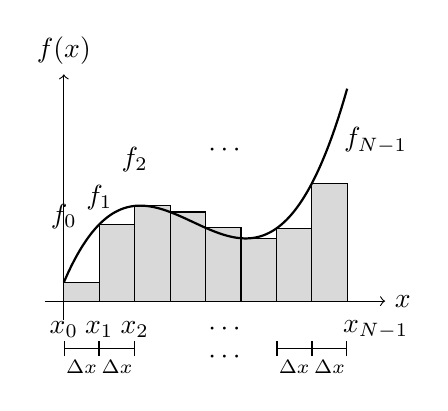
\begin{tikzpicture}[scale=1.2]
			% Ejes
			\draw[->] (-0.2,0) -- (3.4,0) node[right] {$x$};
			\draw[->] (0,-0.2) -- (0,2.4) node[above] {$f(x)$};
			
			% Rectángulos (lower sum)
			\foreach \k in {0,...,7} {
				\pgfmathsetmacro\xleft{0.375*\k}
				\pgfmathsetmacro\xright{0.375*(\k+1)}
				\pgfmathsetmacro\yval{((\xleft - 0.7)^3)/2 - (\xleft - 0.7)^2 + (\xleft - 0.7)/5 + 1}  % Usar el valor en xleft con 0.7
				\draw[fill=gray!30, draw=black] (\xleft,0) rectangle (\xright,\yval);
			}
			
			% Curva original
			\draw[thick, domain=0:3, smooth, samples=100]
			plot(\x, {((\x - 0.7)^3)/2 - (\x - 0.7)^2 + (\x - 0.7)/5 + 1});
			
			% Etiquetas f_k
			\node at (0,0.9) {$f_0$};
			\node at (0.375,1.1) {$f_1$};
			\node at (0.75,1.5) {$f_2$};
			\node at (1.7,1.6) {$\cdots$};
			\node at (3.3,1.7) {$f_{N-1}$};
			
			% Etiquetas x_k
			\node at (0,-0.3) {$x_0$};
			\node at (0.375,-0.3) {$x_1$};
			\node at (0.75,-0.3) {$x_2$};
			\node at (1.7,-0.3) {$\cdots$};
			\node at (3.3,-0.3) {$x_{N-1}$};
			
			% Delta x con fuente más pequeña
			\foreach \k in {0,1,6,7} {
				\pgfmathsetmacro\xstart{0.375*\k}
				\pgfmathsetmacro\xend{0.375*(\k+1)}
				\pgfmathsetmacro\xmid{(\xstart+\xend)/2}
				\draw[|-|] (\xstart,-0.5) -- (\xend,-0.5);
				\node at (\xmid,-0.7) {\scriptsize $\Delta x$};
			}
			
			% Puntos suspensivos en medio
			\node at (1.7,-0.6) {$\cdots$};
		\end{tikzpicture}
		
	\end{minipage}
	\begin{minipage}{0.32\textwidth}
		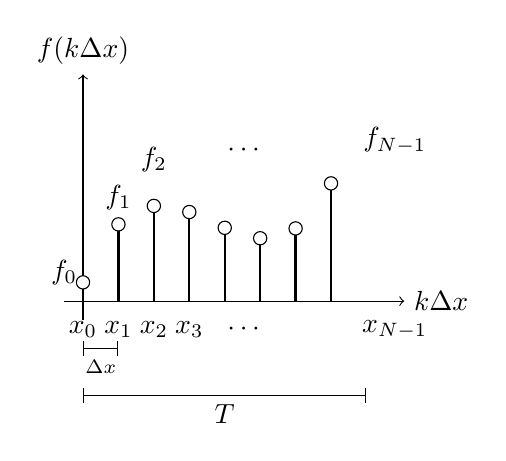
\begin{tikzpicture}[scale=1.2]
			% Ejes
			\draw[->] (-0.2,0) -- (3.4,0) node[right] {$k\Delta x$};
			\draw[->] (0,-0.2) -- (0,2.4) node[above] {$f(k\Delta x)$};
			
			% Stems (discrete samples)
			\foreach \k in {0,...,7} {
				\pgfmathsetmacro\x{0.375*\k}
				\pgfmathsetmacro\y{((\x - 0.7)^3)/2 - (\x - 0.7)^2 + (\x - 0.7)/5 + 1}
				\draw[thick] (\x,0) -- (\x,\y);
				\filldraw[fill=white] (\x,\y) circle (2pt);
			}
			
			% Etiquetas f_k
			\node at (-0.2,0.3) {$f_0$};
			\node at (0.375,1.1) {$f_1$};
			\node at (0.75,1.5) {$f_2$};
			\node at (1.7,1.6) {$\cdots$};
			\node at (3.3,1.7) {$f_{N-1}$};
			
			% Etiquetas x_k abajo
			\node at (0,-0.3) {$x_0$};
			\node at (0.375,-0.3) {$x_1$};
			\node at (0.75,-0.3) {$x_2$};
			\node at (1.125,-0.3) {$x_3$};
			\node at (1.7,-0.3) {$\cdots$};
			\node at (3.3,-0.3) {$x_{N-1}$};
			
			% Marca de Delta x (solo una, inicial)
			\draw[|-|] (0,-0.5) -- (0.375,-0.5);
			\node at (0.1875,-0.7) {\scriptsize $\Delta x$};
			
			% Marca del periodo T
			\draw[|-|] (0,-1) -- (3,-1);
			\node at (1.5,-1.2) {$T$};
		\end{tikzpicture}
	\end{minipage}
\end{center}

\subsection{Transformada Discreta de Fourier (DFT)}

Discretizando la integral (como una suma de Riemann) para los \( N \) valores, tenemos:

\begin{align}
	F_n = C_n &= \frac{1}{T} \int_0^T f(x) \, e^{-i n \frac{2\pi}{T} x} \, dx \\[1ex]
	&\approx \frac{1}{N\Delta x} \sum_{k=0}^{N-1} f(x_k) \, e^{-i n \frac{2\pi}{N\Delta x} k \Delta x} \, \Delta x \\[1ex]
	&= \frac{1}{N} \sum_{k=0}^{N-1} f_k \, e^{-i n \frac{2\pi}{N \Delta x} k \Delta x} \\[1ex]
	&= \frac{1}{N} \sum_{k=0}^{N-1} f_k \, e^{-i n \frac{2\pi}{N} k}
\end{align}

La DFT transforma una secuencia de tiempo discreta en una secuencia de frecuencias discretas.

\[
F_n = \frac{1}{N} \sum_{k=0}^{N-1} f_k e^{-i \frac{2\pi}{N} nk}, \quad n = 0, 1, \ldots, N-1
\]

\subsection{Transformada Inversa Discreta de Fourier (IDFT)}

La transformada inversa permite recuperar las muestras originales, partimos de la serie compleja de Fourier:

\begin{align}
	f_k = f(x) &= \sum_{n=-\infty}^{\infty} C_n \, e^{i n \frac{2\pi}{T} x} \\[1ex]
	&\approx \sum_{n=0}^{N-1} C_n \, e^{i n \frac{2\pi}{N \Delta x} k \Delta x} \\[1ex]
	&= \sum_{n=0}^{N-1} C_n \, e^{i n \frac{2\pi}{N} k}
\end{align}


La transformada inversa permite recuperar las muestras originales:

\[
f_k = \sum_{n=0}^{N-1} F_n e^{i \frac{2\pi}{N} nk}, \quad k = 0, 1, \ldots, N-1
\]

\subsection{Periodicidad de la Transformada Discreta de Fourier (DFT)}

Queremos demostrar que \( F_{n+N} = F_n \). Partimos de la definición:

\begin{align}
	F_{n+N} &= \frac{1}{N} \sum_{k=0}^{N-1} f_k \, e^{-i \frac{2\pi}{N} (n+N)k} \\[1ex]
	&= \frac{1}{N} \sum_{k=0}^{N-1} f_k \, e^{-i \frac{2\pi}{N} nk} \cdot e^{-i \frac{2\pi}{N} Nk} \\[1ex]
	&= \frac{1}{N} \sum_{k=0}^{N-1} f_k \, e^{-i \frac{2\pi}{N} nk} \cdot e^{-i 2\pi k} \\[1ex]
	&= \frac{1}{N} \sum_{k=0}^{N-1} f_k \, e^{-i \frac{2\pi}{N} nk} \quad \text{(ya que \( e^{-i 2\pi k} = 1 \))} \\[1ex]
	&= F_n
\end{align}

Por lo tanto:

\[
F_{n+N} = F_n
\]

La DFT es periódica con periodo \( N \).


\subsection{Periodicidad de la Transformada Inversa Discreta de Fourier (IDFT)}

Queremos demostrar que \( f_{k+N} = f_k \). Partimos de la definición:

\begin{align}
	f_{k+N} &= \sum_{n=0}^{N-1} F_n \, e^{i \frac{2\pi}{N} n(k+N)} \\[1ex]
	&= \sum_{n=0}^{N-1} F_n \, e^{i \frac{2\pi}{N} nk} \cdot e^{i \frac{2\pi}{N} nN} \\[1ex]
	&= \sum_{n=0}^{N-1} F_n \, e^{i \frac{2\pi}{N} nk} \cdot e^{i 2\pi n} \\[1ex]
	&= \sum_{n=0}^{N-1} F_n \, e^{i \frac{2\pi}{N} nk} \quad \text{(ya que \( e^{i 2\pi n} = 1 \))} \\[1ex]
	&= f_k
\end{align}

Por lo tanto:

\[
f_{k+N} = f_k
\]

La IDFT también es periódica con periodo \( N \).


\section{Aplicaciones Web}
Una aplicación web es un software que se ejecuta desde un navegador web, como Google Chrome o Firefox. Estas aplicaciones no necesitan instalarse para poder ser utilizadas, ya que al ejecutarse sobre el navegador solo requieren una conexión a una red de internet. Las aplicaciones web están basadas en una arquitectura cliente-servidor (véase la imagen \ref{fig:cliente-servidor}), en la cual el código se divide en dos partes: scripts del lado del cliente y scripts del lado del servidor ~\cite{apliacionWebAmazon}. Estos dos elementos también se conocen como frontend y backend.

\begin{figure}[h]
	\centering	 
	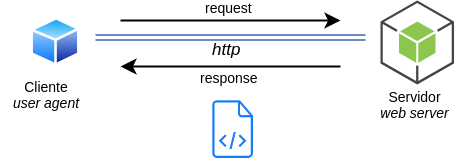
\includegraphics[width=0.9\textwidth]{img/chapter03/ui-web-arquitectura.png}
	\caption[Diagrama de una arquitectura cliente - servidor]{Diagrama de una arquitectura cliente - servidor. \textit{Fuente: ~\cite{uqbar-wiki-web}}}
	\label{fig:cliente-servidor}  % Etiqueta para la figura
\end{figure}


\subsection{Frontend}
El frontend corresponde a la parte del cliente, el cual se encarga de gestionar la funcionalidad de la interfaz de usuario. Cuando el usuario final accede a la aplicación web mediante un enlace, el navegador carga el script del lado del cliente y renderiza tanto los elementos visuales como el texto necesario para la interacción con el usuario. ~\cite{apliacionWebAmazon}.

\subsection{Backend}
El backend corresponde a la parte del lado del servidor, esta se encarga la lógica de la apliación. Este servidor gestiona las solicitudes realizadas por el cliente y devuelve una respuesta. Estas solicitudes pueden incluir acciones como la obtención de datos adicionales, la edición de datos o el almacenamiento de nuevos datos.  ~\cite{apliacionWebAmazon}.
 

\subsection{Tecnologías base de las aplicaciones web}
El desarrollo de aplicaciones web se sustenta en un conjunto de tecnologías fundamentales que permiten crear, diseñar y gestionar tanto el frontend como el backend de dichas aplicaciones. Las 3 tecnologías fundamentales de cualquier apliación web son 3: HTML, CSS y JavaScript.

\subsubsection{HTML}
HTML es el acrónimo de inglés de lenguaje de etiquetas de hipertexto (HyperText Markup Language) es el lenguaje estándar fundamental para estructurar y presentar contenido en la web, siendo la base sobre la cual se construyen todas las páginas web. Su función principal es organizar el contenido de manera semántica, es decir, emplea etiquetas específicas para definir la estructura de los distintos elementos, como encabezados, párrafos, listas, imágenes y enlaces, permitiendo que los navegadores interpreten y muestren adecuadamente el contenido al usuario ~\cite{HTMLMDN}.

\subsubsection{CSS}
CSS es el acrónimo de inglés de hojas de estilo en cascada (Cascading Style Sheets) es básicamente un lenguaje que maneja el diseño y presentación de una aplicación web, es decir, cómo lucen cuando un usuario las visita. Funciona junto con el lenguaje HTML que se encarga del contenido básico de los sitios. Se les denomina hojas de estilo “en cascada” porque se puede tener varias y una de ellas con las propiedades heredadas (o en cascada) de otras ~\cite{CSSMDN}.  

\subsubsection{JavaScript}
JavaScript es un lenguaje de programación que permite brindar interactividad a las aplicaciones web. Desde actualizar fuentes de redes sociales a mostrar animaciones y mapas interactivos, las funciones de JavaScript pueden mejorar la experiencia del usuario de un sitio web. Además, JavaScript funciona como lenguaje de scripting del lado del servidor a través de entornos de ejecución ~\cite{JavascriptMDN}.

\section{API}
API es el acrónimo de inglés de Application Programming Interface (interconexión de programación de aplicaciones), se trata de un softwarae  que permite que sistemas separados compartan información entre sí, actuando como un puente que conecta conecta a la aplicación que envía la solicitud (cliente) con un servidor que le proporciona una respuesta~\cite{APIDazzet}. 

\subsection{API Rest}
Las API de REST (Representational State Transfer o Transferencia del Estado de representación, por su acrónimo del inglés) siguen un conjunto de reglas que hacen que este tipo de API sea mucho más fácil de trabajar; en el núcleo, una API de REST requiere URLs que respondan a las solicitudes HTTP con un elemento de datos o un recurso. Estos datos regularmente están formateados en el marcado de Javascript (JSON en inglés, o Notación de Objetos Javascript). 

\subsection{Protocolo HTTP}
El HTTP, que viene del acrónimo de inglés de Protocolo de Transferencia de Hiper Texto (HyperText Transfer Protocol) es el protocolo esencial para la transmisión de información en la World Wide Web, facilitando la comunicación entre servidores, clientes y proxies mediante un lenguaje común que opera principalmente a través de los puertos 80 y 8080. Al ser un protocolo sin estado, no guarda registro de interacciones anteriores, pero utiliza cookies para almacenar información de visitas previas en el cliente. Su funcionamiento se basa en un esquema de petición-respuesta, permitiendo una comunicación eficiente y flexible entre el usuario (como navegadores o rastreadores web) y los servidores web ~\cite{HTTPEditorialEtece}.

\subsubsection{Métodos de petición HTTP}
HTTP define un conjunto de métodos de petición para indicar la acción que se desea realizar para un recurso determinado. Aunque estos también pueden ser sustantivos, estos métodos de solicitud a veces son llamados HTTP verbs ~\cite{HTTP-metodos-MDN}. los códigos de respuesta son 9:
\begin{itemize}
	\item \textbf{GET}: El método GET solicita una representación de un recurso específico. Las peticiones que usan el método GET sólo deben recuperar datos.
	
	\item \textbf{HEAD}: El método HEAD pide una respuesta idéntica a la de una petición GET, pero sin el cuerpo de la respuesta.
	
	\item \textbf{POST}: El método POST se utiliza para enviar una entidad a un recurso en específico, causando a menudo un cambio en el estado o efectos secundarios en el servidor.
	
	\item \textbf{PUT}: El método PUT reemplaza todas las representaciones actuales del recurso de destino con la carga útil de la petición.
	
	\item \textbf{DELETE}: El método DELETE borra un recurso en específico.
	
	\item \textbf{CONNECT}: El método CONNECT establece un túnel hacia el servidor identificado por el recurso.
	
	\item \textbf{OPTIONS}: El método OPTIONS es utilizado para describir las opciones de comunicación para el recurso de destino.
	
	\item \textbf{TRACE}: El método TRACE realiza una prueba de bucle de retorno de mensaje a lo largo de la ruta al recurso de destino.
	
	\item \textbf{PATCH}: El método PATCH es utilizado para aplicar modificaciones parciales a un recurso.
\end{itemize}

\subsubsection{Códigos de estado de respuesta HTTP}
Los códigos de estado de respuesta HTTP indican si se ha completado satisfactoriamente una solicitud HTTP específica ~\cite{HTTP-codigos-MDN}. Las respuestas se agrupan en cinco clases:
\begin{itemize}
	\item \textbf{Respuestas informativas (100–199)}
%	\begin{itemize}
%		\item \textbf{100 Continue}: El cliente puede continuar con su solicitud.
%		\item \textbf{101 Switching Protocols}: El servidor acepta cambiar el protocolo según lo solicitado.
%		\item \textbf{102 Processing}: El servidor ha recibido y está procesando la solicitud, pero aún no hay respuesta disponible.
%	\end{itemize}
	
	\item \textbf{Respuestas satisfactorias (200–299)}
%	\begin{itemize}
%		\item \textbf{200 OK}: La solicitud fue exitosa.
%		\item \textbf{201 Created}: La solicitud fue exitosa y se creó un nuevo recurso.
%		\item \textbf{202 Accepted}: La solicitud ha sido aceptada para procesamiento, pero aún no se ha completado.
%		\item \textbf{203 Non-Authoritative Information}: La información devuelta es de una fuente secundaria.
%		\item \textbf{204 No Content}: La solicitud fue exitosa, pero no hay contenido para enviar en la respuesta.
%		\item \textbf{205 Reset Content}: Instruye al cliente a restablecer el documento que envió esta solicitud.
%		\item \textbf{206 Partial Content}: Respuesta a una solicitud de rango, indicando que se devuelve solo parte del recurso.
%	\end{itemize}
	
	\item \textbf{Redirecciones (300–399)}
%	\begin{itemize}
%		\item \textbf{300 Multiple Choices}: Hay varias opciones para el recurso solicitado.
%		\item \textbf{301 Moved Permanently}: El recurso solicitado ha sido movido permanentemente.
%		\item \textbf{302 Found}: El recurso solicitado se encuentra temporalmente en otra ubicación.
%		\item \textbf{303 See Other}: El cliente debe realizar una solicitud GET a otro URI.
%		\item \textbf{304 Not Modified}: No se ha modificado el recurso desde la última solicitud.
%		\item \textbf{307 Temporary Redirect}: El recurso solicitado se encuentra temporalmente en otra ubicación (sin cambiar el método HTTP).
%		\item \textbf{308 Permanent Redirect}: El recurso solicitado ha sido movido permanentemente (sin cambiar el método HTTP).
%	\end{itemize}
	
	\item \textbf{Errores de los clientes (400–499)}
%	\begin{itemize}
%		\item \textbf{400 Bad Request}: La solicitud tiene una sintaxis incorrecta.
%		\item \textbf{401 Unauthorized}: La autenticación es necesaria para completar la solicitud.
%		\item \textbf{403 Forbidden}: El servidor entiende la solicitud, pero se niega a autorizarla.
%		\item \textbf{404 Not Found}: El recurso solicitado no se pudo encontrar.
%		\item \textbf{405 Method Not Allowed}: El método HTTP no es permitido para el recurso solicitado.
%		\item \textbf{406 Not Acceptable}: El servidor no puede generar una respuesta en el formato solicitado.
%		\item \textbf{408 Request Timeout}: El servidor agotó el tiempo de espera para la solicitud.
%		\item \textbf{409 Conflict}: Conflicto con el estado actual del recurso.
%		\item \textbf{410 Gone}: El recurso solicitado ya no está disponible y no lo estará nuevamente.
%	\end{itemize}
	
	\item \textbf{Errores de los servidores (500–599)}
%	\begin{itemize}
%		\item \textbf{500 Internal Server Error}: Se produjo un error inesperado en el servidor.
%		\item \textbf{501 Not Implemented}: El servidor no reconoce el método o carece de la capacidad para completarlo.
%		\item \textbf{502 Bad Gateway}: El servidor, actuando como puerta de enlace, recibió una respuesta inválida.
%		\item \textbf{503 Service Unavailable}: El servidor no está disponible temporalmente (sobrecargado o en mantenimiento).
%		\item \textbf{504 Gateway Timeout}: El servidor, actuando como puerta de enlace, no recibió una respuesta oportuna.
%		\item \textbf{505 HTTP Version Not Supported}: El servidor no admite la versión de HTTP utilizada en la solicitud.
%	\end{itemize}
\end{itemize}

\subsection{Tecnologías base para las APIs}
La programación de servicios y microservicios REST simplifica el desarrollo y mantenimiento de aplicaciones web. Sin embargo, su desarrollo y testeo puede resultar incómodo, siempre y cuando, claro está, no se disponga de las herramientas necesarias para el desarrollo de APIs.

\subsubsection{Desarrollo de APIs}
Aunque es perfectamente posible realizar el desarrollo de APIs desde cero, sea cual sea el lenguaje elegido, es conveniente partir de frameworks o plantillas. En algunos casos, serán específicos para el desarrollo de APIs. La lista es interminable y existen para prácticamente todos los lenguajes. 

\subsubsection{NodeJS}
Node.js es un entorno de ejecución de un solo hilo, de código abierto y multiplataforma diseñado para desarrollar aplicaciones de red y del lado del servidor rápidas y escalables de JavaScript (de ahí su terminación en .js haciendo alusión al lenguaje JavaScript). Está escrito en C/C++ y Javascript y emplea una arquitectura de E/S basada en eventos y sin bloqueos, lo que la vuelve eficaz y apropiada para aplicaciones en tiempo real ~\cite{NodeJSKinsta}. 

\begin{figure}[H]
	\centering
	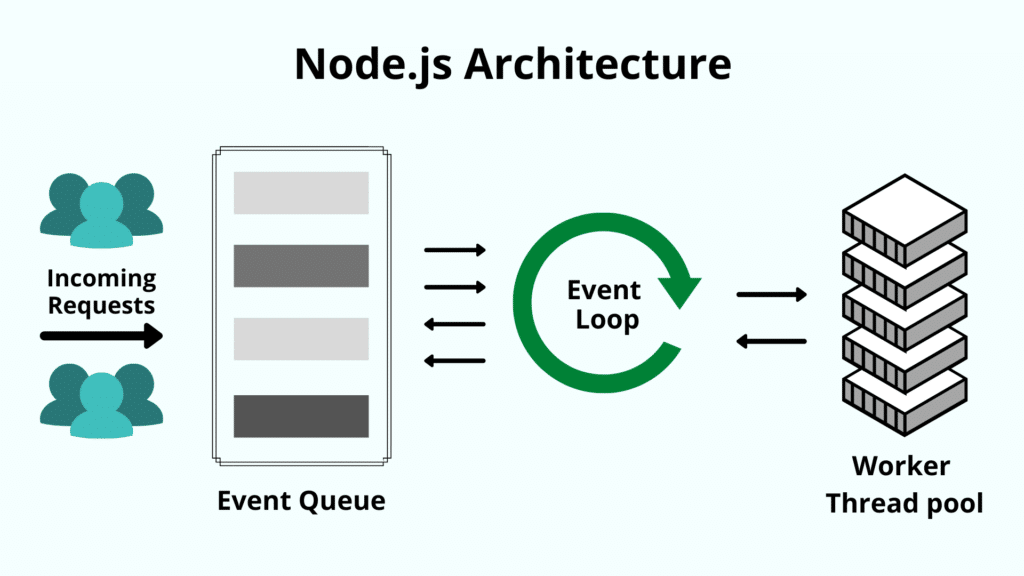
\includegraphics[width=0.8\textwidth]{img/chapter03/node-architecture.png}
	\caption[Cómo procesa node.js las peticiones entrantes utilizando el bucle de eventos]{Cómo procesa node.js las peticiones entrantes utilizando el bucle de eventos. \textit{Fuente: ~\cite{NodeJSKinsta}}}
	\label{fig:nodejs_arqui}  % Etiqueta para la figura
\end{figure}
Node.js utiliza una arquitectura de “Single Threaded Event Loop” \ref{fig:nodejs_arqui} que maneja múltiples solicitudes mediante un único bucle de eventos y un pool de hilos limitado para operaciones de E/S bloqueantes. A diferencia del modelo multihilo de lenguajes como Java, donde cada solicitud se asigna a un hilo individual del pool, Node.js coloca las solicitudes entrantes en una cola y las procesa de manera no bloqueante, asignando hilos del pool de trabajadores solo cuando es necesario. Esta arquitectura reduce el consumo de recursos y memoria, permitiendo una ejecución más rápida de tareas ligeras y haciendo que Node.js sea ideal para aplicaciones en tiempo real. Sin embargo, para tareas que requieren un procesamiento intensivo de datos, los lenguajes multihilo como Java son más adecuados ~\cite{NodeJSKinsta}.
Gracias a su arquitectura, bibliotecas propias de NodeJS como lo es ExpressJS y su amplia demanda en la industria, hacen a NodeJS una gran opción para desarrollar una API.


\subsubsection{Prueba de APIs}
Las herramientas para testear o probar una API son fundamentales para garantizar su máximo desempeño una vez esta sea desplegada. Es importante realizar pruebas de porque garantizan que la comunicación de los datos entre sistemas de software sea precisa. Además, esto ayuda a prevenir inconsistencias de datos o interpretaciones erróneas. Los desarrolladores de API están trabajando en nuevas funciones, mejoras, así como corrección de errores, en consecuencia, las APIs suelen sufrir cambios. Las pruebas de API no solo evalúan las nuevas funcionalidades, sino también aseguran que los nuevos cambios no estén afectando las existentes ~\cite{Postman-QAlified}.

\subsubsection{Postman}
Es una de las herramientas más utilizadas para probar y desarrollar APIs. Permite realizar solicitudes HTTP de manera sencilla y visualizar las respuestas para verificar su precisión. Postman soporta pruebas automatizadas mediante scripts, lo que facilita la validación de la funcionalidad y el rendimiento de la API en diferentes escenarios ~\cite{Postman-QAlified}. 


\section{Seguridad en apliaciones web}
La seguridad en aplicaciones web es fundamental para proteger la integridad, confidencialidad y disponibilidad de los datos manejados, así como para garantizar la confianza de los usuarios. Algunas medidas que se implementan en una aplicación web para implementar dicha seguridad son las siguientes.

\subsubsection{Protocolo HTTPS}
El protocolo de transferencia de hipertexto seguro, por sus siglas en inglés, (HyperText Transfer Protocol Secure) es una versión segura del protocolo HTTP que utiliza el SSL\slash TLS para cifrado y autenticación. HTTPS está especificado por RFC 2818~\cite{RFC2818} y utiliza el puerto 443 o el 8443 de forma predeterminada en lugar del puerto 80/8080 de HTTP ~\cite{HTTPS-SSL}. \newline
HTTPS se diferencia de HTTP al agregar cifrado, autenticación e integridad al protocolo original. Mediante SSL/TLS, HTTPS cifra los datos para protegerlos de interceptaciones y ataques de intermediarios, utilizando criptografía de clave pública para establecer una conexión segura entre el servidor y el navegador. Además, HTTPS autentica la identidad del servidor mediante certificados digitales emitidos por autoridades de certificación confiables, garantizando que los documentos provienen de una fuente legítima. También asegura la integridad de los datos mediante firmas digitales que verifican que el contenido no ha sido alterado durante la transmisión. Estas mejoras hacen que HTTPS sea un protocolo mucho más seguro para navegar y realizar transacciones en la web en comparación con HTTP ~\cite{HTTPS-SSL}, además de volverse un estándar oara cualquier sitio web, ya sea que este intercambie o no datos sensibles con los usuarios.

\subsubsection{Certificado SSL/TLS}
El certificado SSL (Secure Sockets Layer) es una pieza clave para establecer una conexión segura entre el servidor y el cliente. Este establece un enlace cifrado entre un servidor y un cliente. Esto permite que información confidencial se transmita de forma segura a través de Internet.El certificado contiene una clave pública que autentica la identidad del sitio web y permite la transferencia de datos cifrados mediante criptografía asimétrica o de clave pública. La clave privada correspondiente se mantiene en secreto en el servidor ~\cite{SSL-TLS}.

\subsection{CORS}
CORS (Cross-Origin Resource Sharing) es un mecanismo de seguridad usado en los navegadores web que permite a un servidor indicar qué dominios pueden acceder a sus recursos. Por defecto, debido a la política de seguridad del mismo origen, los navegadores restringen las solicitudes HTTP realizadas desde scripts a un dominio diferente al de la página que los ejecuta. CORS agrega encabezados HTTP que indican a los navegadores que permitan a una aplicación web ejecutarse en un origen y acceder a recursos de otro origen diferente. Este tipo de acción se denomina una solicitud HTTP de origen cruzado ~\cite{CORS}.

\section{Frameworks}
Los frameworks son un conjunto de herramientas, estilos y bibliotecas dispuestas a través de una estructura o esqueleto base, para el desarrollo de aplicaciones web más escalables y sencillas de mantener. Son ampliamente utilizados puesto que permiten acelerar el trabajo, reducir los errores, fomentar la colaboración, y obtener un resultado de más calidad. Consiguiendo así que cualquier proceso de trabajo sea más rápido y eficaz, manteniendo la misma calidad. De este modo, gracias a los frameworks web, es posible ahorrar grandes cantidades de tiempo y costes.

\subsection{Angular}
Angular es un Framework de JavaScript de código abierto escrito en TypeScript. Su objetivo principal es desarrollar aplicaciones de una sola página. Google se encarga del mantenimiento y constantes actualizaciones de mejoras para este framework ~\cite{AngularDOCS}. Angular es un framework popular debido a su arquitectura basada en componentes, que permite la reutilización de código y facilita el mantenimiento de aplicaciones grandes y complejas. Además, su potente sistema de enlazado de datos bidireccional (two-way data binding) sincroniza automáticamente la interfaz de usuario con los datos subyacentes, mejorando la experiencia del usuario y la eficiencia en el desarrollo ~\cite{AngularDOCS}.


\subsubsection{TypeScript}
TypeScript es un superset de JavaScript que añade tipado estático y características avanzadas al lenguaje de programación. Desarrollado por Microsoft, TypeScript se compila a JavaScript, lo que permite utilizar sus funcionalidades en cualquier entorno que soporte JavaScript. Al incorporar tipos estáticos, TypeScript facilita la detección temprana de errores durante el desarrollo, mejora la legibilidad del código y facilita el mantenimiento de proyectos a gran escala. Además, ofrece soporte para programación orientada a objetos y otras mejoras que potencian la productividad y la robustez de las aplicaciones web~\cite{TypescriptDOCS}.


\subsubsection{Tailwind CSS}
Tailwind CSS es un framework de CSS  que permite a construir interfaces de usuario personalizadas de manera rápida y eficiente. A diferencia de los frameworks tradicionales que proporcionan componentes predefinidos, Tailwind ofrece clases de utilidad que pueden combinarse directamente en el HTML sin necesidad de escribir CSS personalizado. Esto facilita la creación de diseños responsivos y altamente personalizables, promoviendo la consistencia y reduciendo la cantidad de código CSS necesario~\cite{TailwindCSS}.

\section{Sistema de álgebra computacional}
Un Sistema de Álgebra Computacional (CAS acrónimo del inglés Computer Algebra System) es un software que facilita las operaciones matemáticas y el cálculo simbólico, es decir, cálculos matemáticos usando valores simbólicos (variables y expresiones) en lugar de valores numéricos ~\cite{MaximaSourgeforce}.

\subsection{Maxima}
Maxima es un Sistema de Álgebra Computacional (CAS, por sus siglas en inglés: Computer Algebra System) diseñado en Lisp, de código abierto diseñado para realizar manipulaciones simbólicas y numéricas de expresiones matemáticas. Originalmente desarrollado a partir de una versión de Macsyma del MIT en 1982, Maxima ha evolucionado gracias a la contribución de una comunidad de desarrolladores y usuarios que continúan mejorándolo y ampliando sus capacidades ~\cite{MaximaSourgeforce}.  \newline
Se destaca por ser muy rápido y ligero, lo que permite realizar manipulaciones simbólicas y numéricas de manera eficiente, incluyendo simplificación, derivadas, integrales y resolución de ecuaciones algebraicas y diferenciales. Además, maneja operaciones avanzadas con matrices y vectores, genera gráficos bidimensionales y tridimensionales, y ofrece un lenguaje de programación propio para automatizar cálculos y crear scripts personalizados ~\cite{MaximaSourgeforce}. 

\section{Gráficos en aplicaciones web}
Los gráficos en las aplicaciones web se vuelven necesarios cuando hay que representar visualmente datos y mejorar la interacción del usuario. A través de gráficos, es posible mostrar información compleja de manera intuitiva, facilitando el análisis y la comprensión de los datos por parte de los usuarios. Los gráficos también permiten crear visualizaciones interactivas que enriquecen la experiencia de usuario, proporcionando funciones como zoom, desplazamiento, y selección de datos en tiempo real. Existen diversas herramientas y bibliotecas que permiten generar gráficos avanzados y personalizables para una amplia variedad de aplicaciones web.

\subsection{Canvas}
El elemento \texttt{<canvas>} es una etiqueta de HTML que permite dibujar gráficos, crear animaciones y renderizar imágenes en tiempo real a través de scripting. El elemento \texttt{<canvas>} es sólo un contenedor de gráficos. Es necesario usar JavaScript para crear los gráficos. Canvas cuenta con varios métodos para dibujar trazados, cuadros, círculos, texto así como agregar imágenes. Canvas también es compatible con todos los principales navegadores ~\cite{CanvasHTMLW3S}.  

\section{Representación y captura de funciones matemáticas en sitios web}
Cuando se trata de visualizar elementos que incluyen notación matemática como fórmulas y expresiones algebraicas, es importante utilizar herramientas que permitan renderizar estas expresiones de manera que sea compatible en distintos navegadores, además de facilitar al usuario poder interpretarlos. Esto ayuda a comunicar conceptos complejos de forma clara y accesible, especialmente en aplicaciones educativas o científicas o financieras. Para ello, existen bibliotecas, que permiten tanto la captura como la visualización de fórmulas matemáticas, facilitando la interacción y manipulación de expresiones directamente en el navegador.

\subsection{MathQuill}
MathQuill es un editor de fórmulas de código abierto para la Web mantenido por Mary Stufflebeam y Han Seoul-Oh. Este editor funciona como una biblioteca que importa módulos necesarios para generar un campo de entrada para el usuario, en donde puede escribir expresiones matemáticas de forma que la notación matemática se mantenga lo mejor posible, ya que usa Latex para mostrar los valores ingresados ~\cite{mathquill}. 

\subsection{MathJax}
MathJax es un motor de visualización en JavaScript para notación matemática en LaTeX, que facilita la inclusión de expresiones matemáticas en aplicaciones web sin necesidad de instalar plugins o software adicional. Permite fórmulas en diversos formatos y genera resultados en HTML, CSS o SVG, lo cual asegura que las matemáticas sean textuales y, por tanto, indexables y accesibles en motores de búsqueda ~\cite{mathjax}.

\section{Parsing}
El parsing o parseo es un proceso que implica que un programa analice una cadena de texto, divida sus elementos y extraiga información de utilidad de la misma. Una aplicación del parsing, es el de leer una cadena en determinado lenguaje para convertirlo o entregar una equivalencia del mismo en otro lenguaje.

\subsection{text2max}
Se trata de una biblioteca de código abierto desarrollada por André Storhaug, un estudiante de doctorado en Ciencias de la Computación en la Universidad Noruega de Ciencia y Tecnología (NTNU) ~\cite{Parser-tex2maxima}. Esta biblioteca está desarrollada en Javascript y permite hacer el proceso de parseo entre la sintaxis de \LaTeX a el lenguaje del CAS Maxima.

\section{Servicios de Nube}
Los servicios de nube, también conocidos como \textit{cloud services}, son recursos informáticos que se ofrecen a través de Internet. Estos servicios permiten almacenar, gestionar y procesar datos de manera remota, eliminando la necesidad de infraestructura física local. Los principales beneficios de los servicios de nube incluyen escalabilidad, flexibilidad, accesibilidad desde cualquier ubicación, y reducción de costos operativos. Además, facilitan la colaboración y el acceso a aplicaciones y herramientas avanzadas sin requerir instalaciones complejas, lo que los hace fundamentales para el desarrollo y despliegue de aplicaciones web modernas ~\cite{microsoft_azure}.

\subsection{Microsoft Azure}
Microsoft Azure es una plataforma de servicios en la nube proporcionada por Microsoft, que ofrece una amplia gama de soluciones para computación, almacenamiento, bases de datos, análisis, redes, inteligencia artificial y más. Azure permite a los desarrolladores crear, desplegar y gestionar aplicaciones de manera eficiente utilizando herramientas y frameworks familiares. Además, Azure garantiza alta disponibilidad, seguridad robusta y cumplimiento de normativas, lo que lo convierte en una opción confiable para empresas de todos los tamaños ~\cite{microsoft_azure}´. 

\section{Interfaz gráfica de usuario}
Las Interfaces Gráficas de Usuario (GUI) son omnipresentes en nuestra vida cotidiana, ya sea al utilizar una computadora o un celular entre otros dispositivos. La eficacia de una GUI es crucial para determinar si un producto será competitivo o no. Un producto puede fracasar si el usuario no logra completar una acción, como una transacción económica, si no comprende la secuencia de pasos requeridos, si no encuentra fácilmente cómo realizar una acción necesaria, como hacer una compra, o si no encuentra atractivo el diseño de la aplicación ~\cite{interfazAlbornoz}.
\subsection{Principios de Usabilidad}
Los principios de usabilidad web son la base de cualquier página web para que sea “user friendly”. O lo que es lo mismo, es un tipo de diseño centrado en el usuario para conseguir mejorar la experiencia del mismo. La usabilidad se refiere a la facilidad con la que los usuarios interactúan con una herramienta con el fin de lograr un propósito específico. Así pues, la usabilidad web indica hasta qué punto un sitio web resulta sencillo de utilizar. Esto significa que para que una apliación web ~\cite{usabilidadJakob}. \newline
Los principios de usabilidad, son diez fundamentos que facilitan el diseño de productos más aceptados por los usuarios al enfocarse en sus necesidades y comportamientos~\cite{usabilidadJakob}:
\begin{enumerate}
	\item \textbf{Visibilidad del estado del sistema.} El usuario siempre debe de estar informado de lo que está pasando en en la aplicación web y ofrecerle una respuesta en el menor tiempo posible. Ejemplos de esto son las barras de carga o notificaciones sobre el navegador.
	
	\item \textbf{Relación entre el sistema y el mundo real.} El sistema tiene que “hablar” el lenguaje del usuario usando palabras, frases inclusive símbolos con los que el esté familiarizado y que pueda reconocer con facilidad. Para esto la información debe mostrarse en un orden lógico y usando las palabras y símbolos correctos, sin darle oportunidad al usuario de equivocarse.
	\item \textbf{Control y libertad del usuario.} Los usuarios pueden equivocarse al realizar una acción dentro de la apliación, así que este debe tener la oportunidad de corregir su error y no sentirse frustrado por ello. Claro ejemplo de esto es un botón de deshacer.
	
	\item \textbf{Consistencia y estándares.} Las aplicaciones deben de seguir los estándares y convenios establecidos para iconos o colores, por ejemplo un icono con lineas verticales indica un menú, o el color verde y rojo se asocian con aceptar y cancelar, respectivamente.
	
	\item \textbf{Prevención de errores.} La apliación debe de prevenir cualquier posible error que el usuario pueda cometer, y encaso de que este cometa uno, debe de disponer de diversas herramientas para corregirlo, limitar caracteres o entradas no validas por el sistema es un ejemplo de esto.
	
	\item \textbf{Reconocer antes que recordar.} La apliación debe ayudar al usuario a no tener que memorizar acciones u objetos para que pueda usarla fácilmente, usar botones asignados y personalizados para acciones especificas es un ejemplo de esto.
	
	\item \textbf{Flexibilidad y eficiencia de uso.} La apliación debe de de estar preparada para recibir a todo tipo de usuarios, si alguien inexperto en el sitio o en el tema del mismo se pueden brindar ayudas como ventanas con mensajes o tutoriales. 
	
	\item \textbf{Diseño estético y minimalista.} La apliación no debe de tener información innecesaria que distraiga al usuario y perturbe su experiencia al usarla.
	
	\item \textbf{Ayudar a los usuarios a reconocer, diagnosticar y corregir los errores.} En caso de que se produzca un error o excepción dentro de la aplicación, los mensajes de error deben ser compresibles para el usuario, como pasar de un ERROR 404 a un mensaje mas entendible como ERROR DEL SERVIDOR.
	
	\item \textbf{Ayuda y documentación.} Es preciso que la apliación cuente con un manual de funcionamiento, esto ayuda al usuario a que le sea mas fácil usar la apliación. Este manual debe ser facil de localizar, definir los pasos claramente y no de manera extensa.
\end{enumerate}

El cumplir con estos principios de usabilidad ayudan a que el sitio cuente con un trafico más recurrente, es decir, aumentamos las posibilidades de que un usuario, después de utilizar la apliación, la vuelva a usar en un futuro, así como que más personas la usen, demás de que se disminuye el porcentaje de rebote, que no es otra cosa que conseguir que el tiempo de estancia del usuario en la aplicación sea más alto y que explore mas partes del sitio.


 
%\subsubsection{Introducción a NodeJS}
%Explicación básica sobre NodeJS.
%\subsubsection{Ventajas del uso de NodeJS para aplicaciones web}
%Descripción de por qué se eligió NodeJS para la parte del servidor.
%\subsubsection{Integración de NodeJS con Maxima}
%Detalle de cómo se usa NodeJS para comunicarse con Maxima y realizar cálculos matemáticos.

%\subsubsection{Qué es Maxima y por qué se usa para cálculos simbólicos}
%Explicación sobre el software Maxima y su importancia en los cálculos de Series de Fourier. 
%\subsubsection{Implementación de Maxima en el servidor}
%Cómo se utiliza Maxima en el servidor junto con NodeJS para realizar cálculos matemáticos de forma eficiente.

%
%
%\section{Recommendations and future work}
%\begin{table}[hbtp]
%	\centering
%	\begin{tabular}{@{}*{2}{p{0.5\textwidth}}@{}}
%		\toprule
%		\textbf{Correct} &  \textbf{Incorrect}
%		\\
%		\midrule
%		\enquote{This is an \enquote{inner quote} inside an outer quote}
%		&
%		"This is an 'inner quote' inside an outer quote"
%		\\
%		\bottomrule
%	\end{tabular}
%	\caption[Quotation marks]
%	{Proper quotation mark usage.
%		The \texttt{\textbackslash enquote} command chooses the correct
%		quotation marks for the specified language.}
%\end{table}
%\lipsum[1]